\documentclass[12pt,BSc,wordcount]{muthesis}

\usepackage{url} % typeset URL's sensibly

\usepackage{pslatex} % Use Postscript fonts

\usepackage{minted}
\usemintedstyle{emacs}

\usepackage{float}

\usepackage[caption = false]{subfig}

\usepackage{graphicx}

\usepackage{listings}

\usepackage[hidelinks]{hyperref}

\usepackage{dirtree}

\usepackage{verbatim}

%% Cound listing with chapter numbers
\usepackage{chngcntr}
\counterwithin{listing}{chapter}

\usepackage[utf8]{inputenc}
\usepackage{glossaries}

\usepackage{csquotes}

%% Use BibLatex
\usepackage[
backend=biber,
style=ieee,
sorting=nty,
defernumbers=true
]{biblatex}
\addbibresource{refs.bib}

%% Patch the @online bib citation to not include empty parenthesis when
%% No date is given
%% https://tex.stackexchange.com/questions/151217/remove-parentheses-for-empty-year-field-biblatex-ieee-style
\usepackage{xpatch}
\xpatchbibdriver{online}
  {\printtext[parens]{\usebibmacro{date}}}
  {\iffieldundef{year}
    {}
    {\printtext[parens]{\usebibmacro{date}}}}
  {}
  {\typeout{There was an error patching biblatex-ieee (specifically, ieee.bbx's @online driver)}}

% Uncomment the next line if you want subsubsections to be numbered
\setcounter{secnumdepth}{3}
% Uncomment the next line if you want subsubsections to be appear in
% the table of contents
\setcounter{tocdepth}{3}

% Uncomment the following lines if you want to include the date as a
% header in draft versions
\usepackage{fancyhdr}
\pagestyle{fancy}
\lhead{}  % left head
\chead{Draft: \today} % centre head
\lfoot{}
\cfoot{\thepage}
\rfoot{}

% Include glossary terms
\makeglossaries

\newglossaryentry{domain_expert}
{
    name={domain expert},
    description={An individual who deeply understands a particular subject matter or domain, such as healthcare, finance, or marketing, possessing extensive knowledge, skills, and experience in the domain}
}

\newglossaryentry{data_lake}
{
    name={data lake},
    description={A centralized repository that allows storing structured and unstructured data at any scale, usually used to run analytics \cite{awsWhatIsADataLake2023}}
}

\newglossaryentry{data_mesh}
{
    name={data mesh},
    description={An extension of the data lake system, with the constraints that domain owners handle their data pipelines themselves, most procedures are self-service and data has to meet higher standards \cite{montecarloDataLakeVSDataMesh2023}}
}

\newglossaryentry{data_silo}
{
    name={data silo},
    description={A collection of data held by one group that is not easily or fully accessible by other groups in the same organization}
}

\newacronym{pii}{PII}{Personally identifiable information}

\newacronym{dbms}{DBMS}{Database management system}

\newacronym{jwt}{JWT}{JSON Web Token}

\newacronym{sso}{SSO}{Single Sign-On}

\begin{document}
    % Uncomment the following lines to leave out the list of figures, tables
    % and copyright until final printing
    %\figurespagefalse
    \tablespagefalse
    %\copyrightfalse
    
    %% This defines the title (the \\ forces a line break)
    \title{Big Data for humans - metadata authorisation with respect to privacy and user information}
    %% and author
    \author{Marius Cristian Osiac}
    \stuid{1464967}
    %% and supervisor
    \principaladviser{Dr Mary McGee Wood}
    
    %% This defines the file that contains the text of the abstract, there
    %% must be one of these by the time you submit your report.
    \beforeabstract
    
    %% Add a list of listing by hand since it's not handeled by the template 
    \addvspace{10pt}
    \listoflistings
    \newpage
    
    \prefacesection{Abstract}
    TODO: Put abstract here
    
    %% This defines the file that contains the acknowledgements (it can be
    %% omitted if you don't feel like thanking anyone
    \prefacesection{Acknowledgements}
    TODO: Add merci page
    \afterpreface
    
    % Add Glossary
    \printglossary
    
    %% These include the actual text
    \chapter{Introduction}
\label{cha:intro}

This report explores the various challenges and solutions related to metadata authorisation and discusses the technical challenges of implementing a robust metadata authorisation system based on industry-standard technologies: OpenMetadata and Apache Ranger.

In the last few decades, the explosion of digital technology has led to an increasing amount of data being collected and generated. The rise of big data has led to many opportunities and challenges for organisations and individuals alike. However, with this abundance of data comes the risk of privacy infringement and the abuse of user information. Metadata has become a critical component in securing individuals' privacy and user information.

Metadata can provide valuable insights into the structure of data and how it is used, but it can also be used to track, identify and monitor individuals without their consent. As such, it is crucial to ensure that system administrators have control over all information about the data their organisation stores and how it is used. This is where metadata authorisation comes into play.

Metadata authorisation is the process of granting or denying access to metadata. It is crucial for any organisation that collects user data to have a robust metadata authorisation system that enables the protection of the privacy and personally-identifying information of individuals while still allowing for the most effective use of data and metadata. Metadata authorisation is crucial in industries such as healthcare, finance, and marketing, where sensitive personal information is frequently collected.

 \section{Background}

 Metadata is "data that provides information about other data", but not directly about the content of the data, such as individual rows in a table or the pixels of an image. Categories of metadata commonly encountered include but are not limited to \cite{understandingMetadataRiley2017}:

\begin{itemize}
    \item Descriptive metadata - relates to finding and comprehending data. As an example, a book may consist of the title, author, subject and ISBN;
    \item Administrative metadata - relates to how the data is intended to be used. Examples of this type are technical metadata (e.g., the format of a file, instructions for decoding), preservation or authenticity metadata (e.g., versioning artefacts, digital signatures, check-sums) and rights of legal metadata (e.g., licensing);
    \item Structural metadata - describing relationships of data to other resources;
    \item Statistical metadata - often used in statistics, describing the procurement, processing and aggregation done to create data sets \cite{roleOfMetadataInStatisticsdippo2000}. 
\end{itemize}

Big data refers to data sets that are too large and complex to be dealt with using traditional data processing methods and software while being at the centre of modern business and science. Until 2003, humans created roughly 5 exabytes ($10^{18}$ bytes) of stored data. In 2013, that amount was generated in two days \cite{bigDataAReviewsagiroglu2013}. Big data is characterised by its three V's \cite{understandingBigDataZikopoulos2011}:

\begin{itemize}
    \item Variety - the structure of data, which comes from many heterogeneous sources in different formats. Data may be structured, when it is warehoused, well organised, tagged and labelled, semi-structured or unstructured, where most data resides, random, difficult and costly to use effectively;
    \item Volume - the size of data, which is always increasing, is larger than the petabyte scale;
    \item Velocity - the speed at which data changes dictates the optimal way to use it. Data may be acquired in batches or arrive as a discrete stream of samples.
\end{itemize}

In the context of Big data, metadata is concerned with what the data is, where it comes from, how it was processed, what is the data type of each of its elements, what units it is measured in, what formulas were used to derive it, who owns it, governance processes. Metadata is a core part of the effective use of big data.

Security is a significant concern in the context of Big Data systems, concerning protecting confidentiality, integrity and data availability. Data centralised in one place opens itself up as a valuable attack target. Big Data privacy is also a relevant matter, concerned with protecting individuals' personal information. These systems commonly store and aggregate large amounts of personally identifying information collected from various sources, so mismanagement can seriously impact the users' privacy \cite{bigDataSecurityTankard20125}. There is an increasing number of regulations organisations handling user data must follow relating to how data is collected and where it is stored and used. For example, the healthcare industry has been adopting the Big Data approach for storing patient records, which are inherently \acrshort{pii} and are heavily regulated, thus privacy in those systems is a major point of contention \cite{bigDataSecurityHealthPatil2014}.

\section{Motivation}

Data is growing exponentially, and soon all data may become Big Data. The Big Data approach has been widely adopted to handle large amounts of data in the computer science world for some time. While not a solved problem, storing large quantities of data has become more manageable with the decrease in the price of storage and processing units and the increase in the popularity of unstructured, file-based storage on distributed systems like AWS's S3, Casandra, and HDFS. Doing large and complex computations on these data sets is extensively aided by the ability to detach computational power from storage, something \acrshort{dbms} are limited by, with \gls{data_mesh} tools such as Trino\footnote{Formerly known as Presto} \cite{trinoTech, trinoSethi2019}, Dremio \cite{dremioTech}, or Apache Drill \cite{apacheDrillTech, apacheDrillHausenblas2013}.

These advancements are significant, but they must address an important point - storage and computing are useless if \glspl{domain_expert} (i.e. not necessarily engineers) cannot use them effectively. Historically, analysts would run queries to gather data, format it, plot graphs, and write articles manually to provide insights. However, the industry is trending more towards automating some of these steps using giant SQL engines or data processing pipelines. Automation has been a significant advancement, but it brought another problem - more derived data is generated, which is very hard to keep track of.

Gathering insights from data is finally a human process, and our goal as engineers should be to assist this process by providing tooling, not to replace people with computers. In a \gls{data_mesh}, \glspl{data_lake} are connected to \glspl{data_lake}, \glspl{data_silo} are connected to other \glspl{data_silo}, comprising structured and unstructured, collected and derived, hand-picked and computer-generated data so it is becoming increasingly hard for \glspl{domain_expert} to find and manage the data sets they are interested in or to discover new ones.

Metadata, data catalogues and data indexing systems are essential tools for data-driven organisations to maintain, govern and use data in the most efficient manner possible by allowing data analysts, data scientists, domain experts and administrators to understand the sprawling \glspl{data_mesh} they are working with. Big Data systems have largely evolved without adjacent metadata management infrastructure, which can, in part, be seen as a good thing, empowering data interoperability and loosening constraints. However, as these systems mature, more advanced and complete solutions are needed to handle "Big Metadata" \cite{bigMetadataSmith2014}. As metadata and data discovery tools evolve, the need to consider the aspects of security, privacy and data access control is becoming more relevant.

\section{Current Solutions}

Open-source metadata catalogues and data discovery systems have gained traction in the previous years, as large companies such as LinkedIn, Lyft and Netflix have internal projects for the public. It is crucial to remember that these projects were created to mould around each organisation's specific workflows and pipelines; thus, these are products of their environments, and the set of features they offer reflects that. Examples of such systems include Amundsen Lyft \cite{amundsenLyftGrover2019}, LinkedIn DatHub \cite{dataHubLinkedinLan2019}, and Netflix Metacat \cite{metacatNetflixMajumdar2018}, which have similar features and functionalities compared to OpenMetadata but, just as similarly, have a lacking approach towards controlling access to metadata.

An outlier in the group of open-source solutions is Apache Atlas \cite{apacheAtlasTech}. Initially incubated by Hortonworks, it is now under the umbrella of the Apache Software Foundation, which, some may argue, positions it at a higher standard of quality compared to the former corporate-owned projects. What makes Apache Atlas an outliner is the organisation backing it but the project's attention to data governance, access control for both data and metadata and privacy of users' data. Apache Atlas is part of the Hadoop ecosystems and natively integrates with Apache Ranger, offering specialised functionality, which we will cover in later parts of the report, Apache Hive, Apache Kafka and others, but is limited in interoperability with systems outside its ecosystems. In this area, the former systems excel.

The realm of data cataloguing systems encompasses a significant portion of commercially available solutions, with Informatica \cite{informaticaTech} being a notable exemplar. However, these solutions are proprietarily licensed, exorbitantly priced, and solely accessible to large-scale organisations. Consequently, assessing their features poses a challenge.

\section{\label{sec:project_goal} Aims and Objectives}

This report aims to examine the current issues of metadata authorisation systems with particular concern towards securing user information and present the design and implementation of a more suitable solution.

The report will explore methods of managing control of access to metadata and metadata governance solutions. The work is done in the context of using OpenMetadata as the metadata store and Apache Ranger as the centralised security framework, with the goal of integrating these two systems.

The report will be looking at OpenMetadata and its main functionalities, what systems for access control are already in place, what their shortcomings are and how these can be expanded. It will review Apache Ranger's functionalities, how its plugins operate, and how a new plugin for OpenMetadata is designed and implemented. Apache Ranger needs to be more well documented, so this report aims to introduce the many parts of Apache Ranger and serve as a general guide for integrating services.

Finally, the project will evaluate the quality of the proposed solution, considering how secure the system is and how well it can protect users' privacy, how flexible the approach is and how easily it can be further extended and the performance impact.

\section{Technologies Used}

OpenMetadata is an open-source platform for metadata management that aims to help data-driven organisations govern their data and metadata in a flexible and extensible way, integrating with many industry-standard tools, processes and technologies. It addresses the challenges faced by organisations with large amounts of sprawling data by providing a centralised platform that handles the management, definition, storage and procurement of the metadata for many different data resources, such as tables, columns, databases, files, dashboards, charts and also for the workflows and processes that resulted in those resources. Relating to the metadata categories described above, OpenMetadata focuses on descriptive and structural but is flexible enough to accommodate any other type. The platform automates the process of metadata discovery and indexing from various sources, such as \glspl{data_lake} (e.g., Trino), databases (e.g., PostgreSQL \cite{postgresqlTech}), business intelligence tools (e.g., PowerBI \cite{powerbiTech}), messaging queues (e.g., Apache Kafka \cite{apacheKafkaTech}), workflow orchestration tools (e.g., Apache Airflow \cite{apacheAirflowTech}). OpenMetadata is designed to be API-first \cite{apiFirstBealieu} so it fully-featured support programmatic access, and provides a user-friendly interface for data consumers, metadata maintainers, and data analysts and scientists to explore data and collaborate.

Apache Ranger \cite{apacheRangerAccessControlModelGuptaMaanak2017,apacheRangerMultiLayerdGuptaMaanak2017} is an open-source security framework for enforcing fine-grained access control policies and auditing access to resources. It was developed by the Apache Foundation to integrate with systems in the Hadoop ecosystem and to tackle the security issues that commonly appear in big data applications. The framework offers a centralised point for security management across a sizeable data-driven organisation where administrators can create data access policies based on user or group permissions or data attributes (also commonly called tags) and comprehensive auditing functionality, empowering the monitoring of resource access and detection of malicious intent. Apache Ranger is widely used in healthcare 
to secure patient records \cite{rangerHealhcareRangarajan2018}, in telecommunications to protect customer information \cite{rangerTelecomAhmad2019} and in finance to comply with regulatory requirements. The framework easily integrates with other systems in the Hadoop ecosystem, such as HDFS \cite{HDFSBorthakur2008}, HBase \cite{apacheHbaseTech}, Solr \cite{apacheSolrTech} and Kafka, but also with components outside of it, such as Trino and Elasticsearch \cite{elasticsearchTech}.

\section{Summary}

The report is structured in the following chapters:

\begin{itemize}
    \item \textbf{Chapter 1: \nameref{cha:intro}} presents an overview of the problem, the motivation behind the project, the aims and objectives and a short introduction of the main technologies used;
    \item \textbf{Chapter 2: \nameref{cha:context}} covers the industry-standard system and technologies that the report builds upon in detail;
    \item \textbf{Chapter 3: \nameref{cha:design}} overviews the high-level architectural design of the proposed metadata authorisation system and illustrates the flow of data and operation in the access control pipeline;
    \item \textbf{Chapter 4: \nameref{cha:impl}} presents the steps taken to implement the proposed system and the challenges encountered in the process and the efforts taken to ensure the solution's flexibility and extensibility;
    \item \textbf{Chapter 5: \nameref{cha:exp}} examines the correctness and performance of the resulting system;
    \item \textbf{Chapter 6: \nameref{cha:conclusion}} encompasses the reflection, conclusion, and future work.
\end{itemize}
    \chapter{\label{cha:context} Technical Background}

This chapter thoroughly discusses the two central systems the project is concerned with: Apache Ranger and OpenMetadat. It will also briefly cover related items, such as building a local debugging harness, Java practices for developing large, distributed and extensible frameworks and dependency management. As mentioned in Section \ref{sec:project_goal}, this chapter aims to present itself as an introduction to the inner working of Apache Ranger and methodologies for expanding its suite of interoperable services.  

\section{Active Directory and Lightweight Directory Access Protocol}

TODO: Add background here.

\section{\label{sec:tech_background_apache_ranger} Apache Ranger}

Terms commonly used from here on out are defined as follows:

\begin{itemize}
    \item \textbf{Service definition} - a definition for a type of service (e.g., Hive, HDFS, HBase) in JSON format;
    \item \textbf{Service} - a connection to an external process using an Apache Ranger plugin to govern access control, comprised of configuration and a list of policies. Configuration is commonly composed of connection parameters, allowing Ranger to communicate with the external process;
    \item \textbf{External user} - an account in the organisation and managed using Active Directory (e.g., LDAP) or Unix-compatible user and group systems. Users have a unique username and are members of a set of groups, which may represent the user's department or permissions;
    \item \textbf{Role} - a shorthand for a specific set of users, groups and other roles that exist only in Ranger (it is not part of the organisation's Active Directory);
    \item \textbf{Resource} - any data, application, or service that needs to be protected and managed by the access control system. Resources can take many forms, such as databases, tables, columns, HDFS paths, Hive queries, Kafka topics, and Elasticsearch topics;
    \item \textbf{Access type} - a way a user can interact with a resource. Common access types are view, edit, create and delete; 
    \item \textbf{Policy} - a rule that describes what access types certain users are permitted to use on a set of resources with a common pattern.
\end{itemize}

\begin{figure}
    \centering
    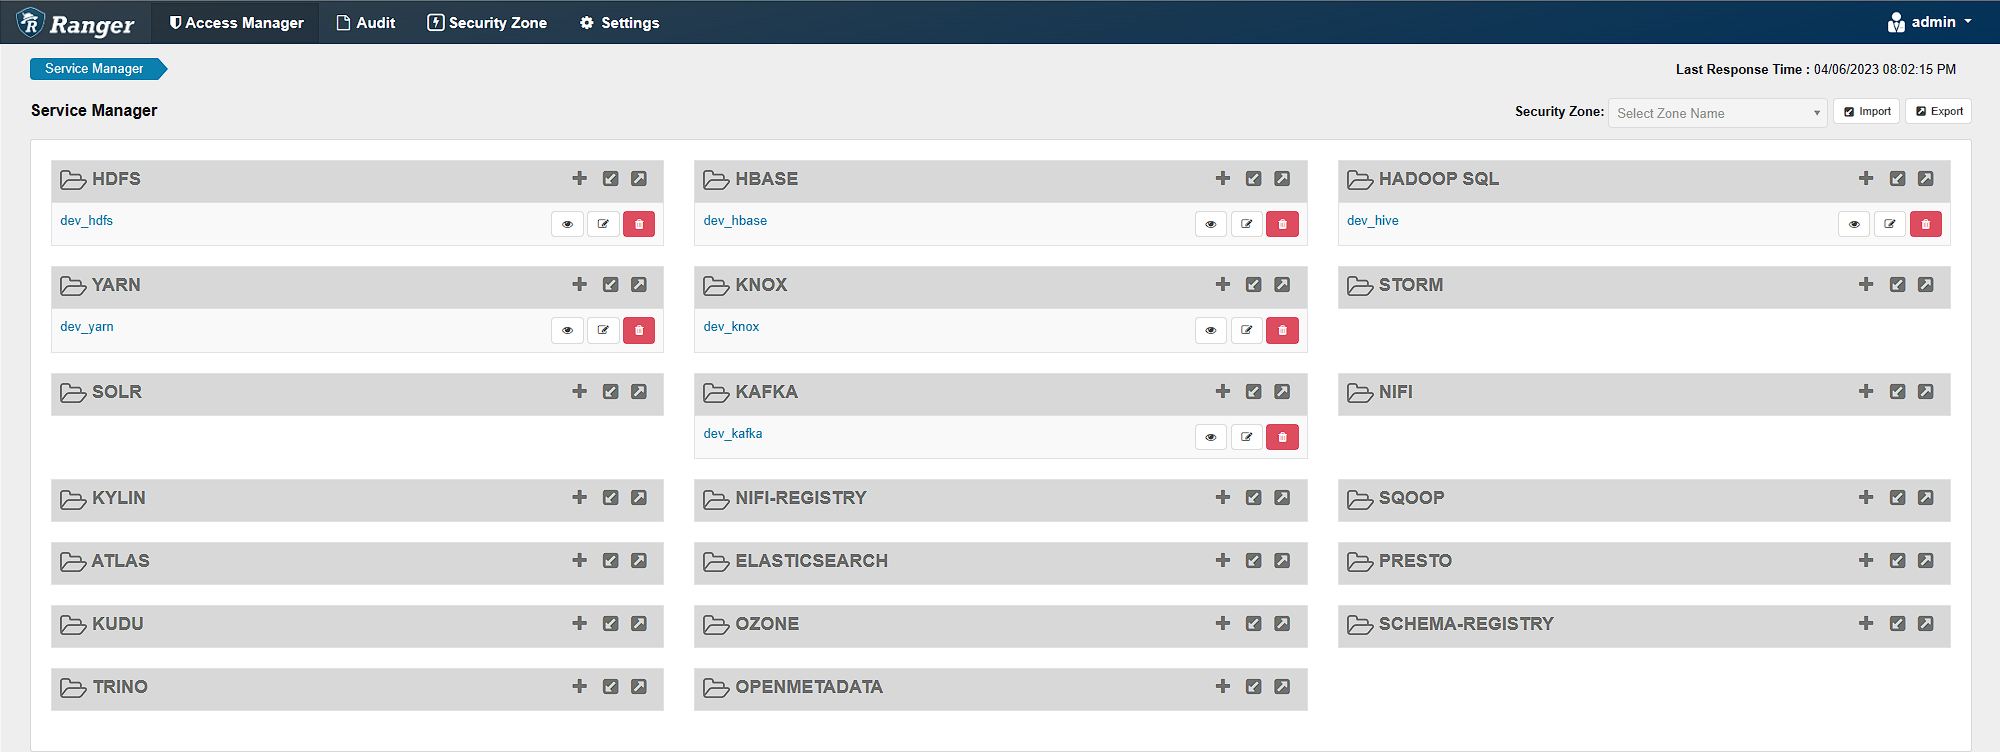
\includegraphics[width=\textwidth]{chapters/tech_background/figures/ranger-admin.png}
    \caption{Landing page for Apache Ranger user interface, showing sample services.}
    \label{fig:ranger-admin}
\end{figure}

\begin{figure}
    \centering
    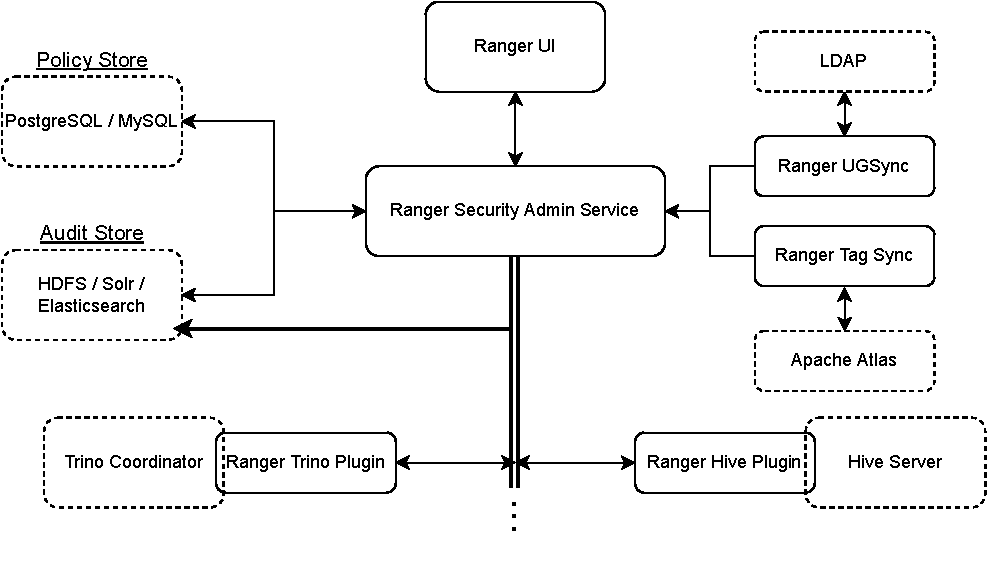
\includegraphics[width=0.8\textwidth]{chapters/tech_background/figures/ranger-arch.pdf}
    \caption{Architectural diagram of the Apache Ranger system.}
    \label{fig:rager_arch}
\end{figure}

All the core components of the Apache Ranger framework are written in Java, originally developed using Java 8, but forwards-compatible with Java 11, and the user interface is written in JavaScript. Apache Maven handles the project's structure and build. It is split into multiple modules, each concerned with different framework parts. We will be looking at \mintinline{java}{security-admin} (also referred to as the security admin service), \mintinline{java}{ugsync} (a short name for user and group sync) and plugins with their respective shims (e.g., \mintinline{java}{plugin-trino} and \mintinline{java}{range-trino-plugin-shim}). Figure \ref{fig:rager_arch} shows an architectural diagram of Apache Ranger's primary components, with full boxes representing first-party components and dashed boxes representing external services.

The \mintinline{java}{security-admin}, along with the user interface, is the heart of the system and the place where admins will define and connect services and manage access policies, security zones and user roles. Figure \ref{fig:ranger-admin} shows the landing page of the user interface, where various demo services have been added.

Figure \ref{fig:ranger_hive} shows the eight default policies created for the \mintinline{java}{dev_hive} service, and Figure \ref{fig:ranger_hive_poly} shows the details of the \mintinline[breaklines]{java}{all - database, table, column} policy, which is defined for resources that follow pattern \mintinline[breaklines]{java}{{database="*", table="*", column="*"}}, which can be read as "all columns, in all tables, in all databases". The policy allows the \mintinline{java}{hive} user to do a subset of all actions. It enables the owner of the resource (\mintinline{java}{{OWNER}} is a macro that is replaced with the owner of the resources at evaluation time) to do all actions on these resources.

The \mintinline{java}{ugservice} is an asynchronous process that monitors an Active Directory or a Unix-compatible user and group systems and populates the security admin service's repository of external users and groups.

\begin{figure}
    \centering
    \subfloat[\centering \label{fig:ranger_hive} All policies created for the \mintinline{java}{dev_hive} Hive service.]{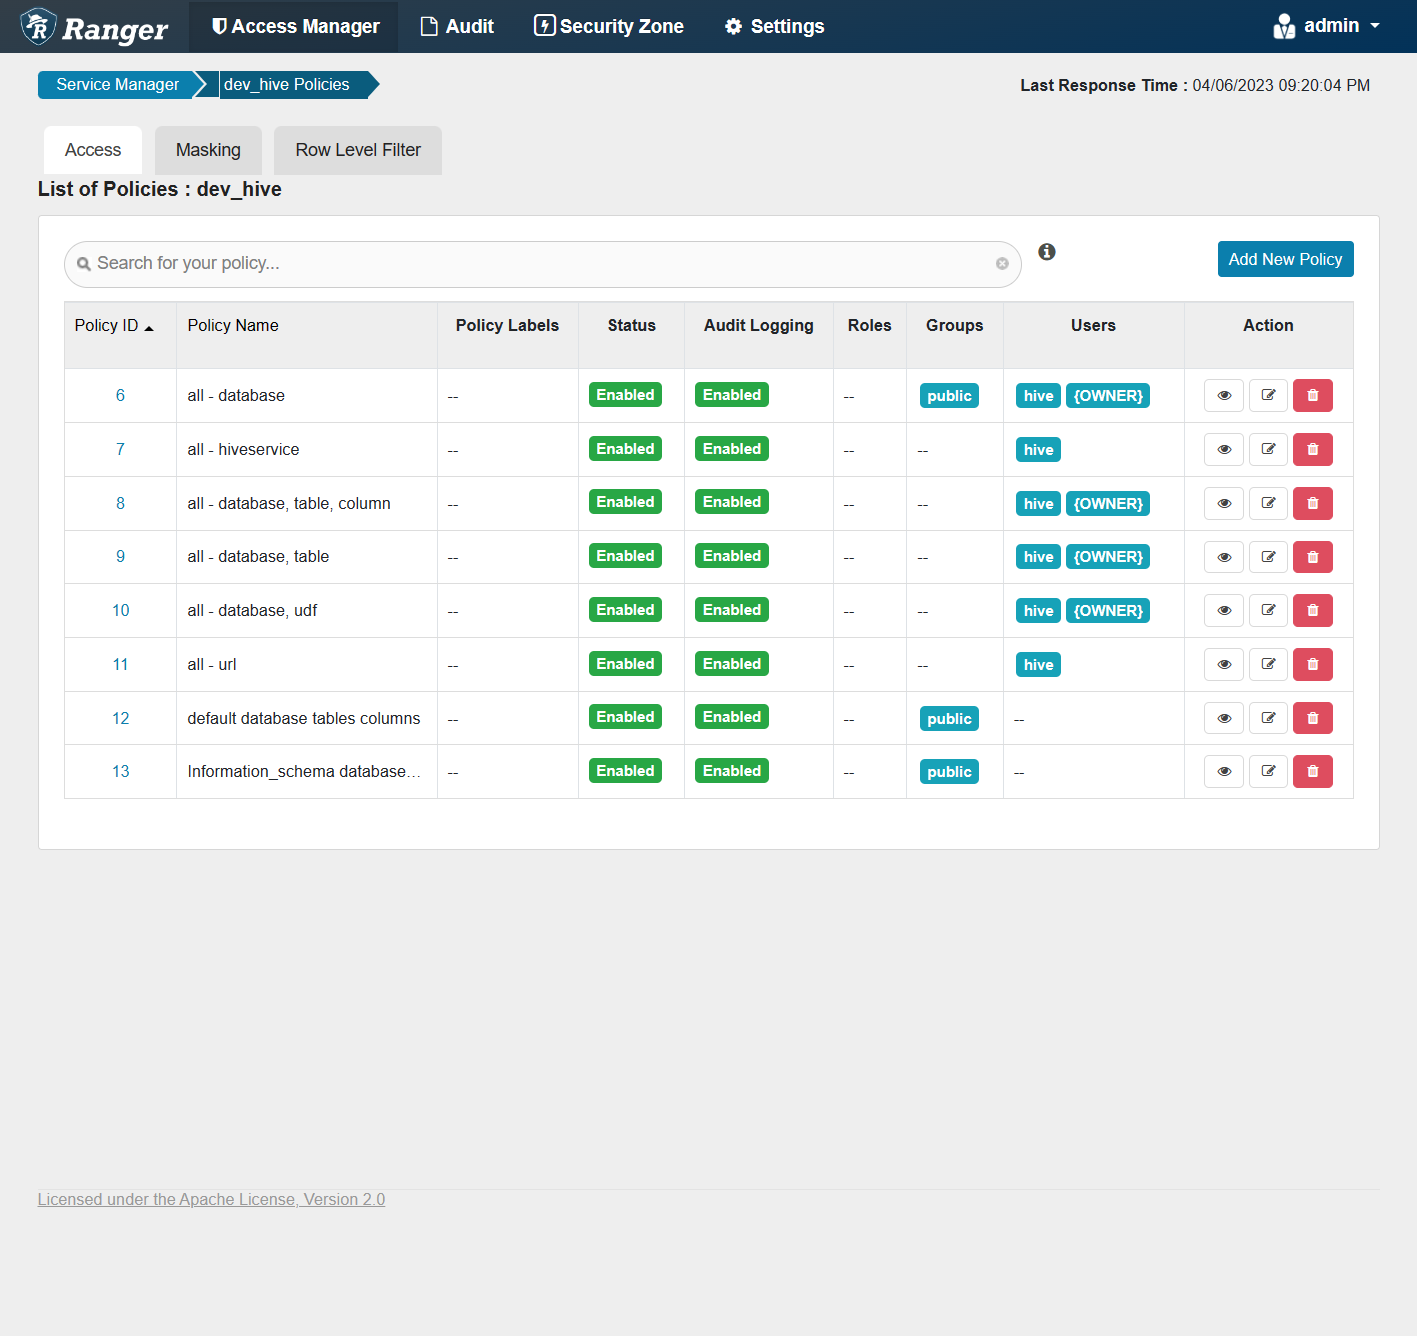
\includegraphics[width=0.65\textwidth]{chapters/tech_background/figures/ranger_hive.png}}
    \qquad
    \subfloat[\centering \label{fig:ranger_hive_poly} The \mintinline{java}{all - database, table, column} policy defined for the Hive service.]{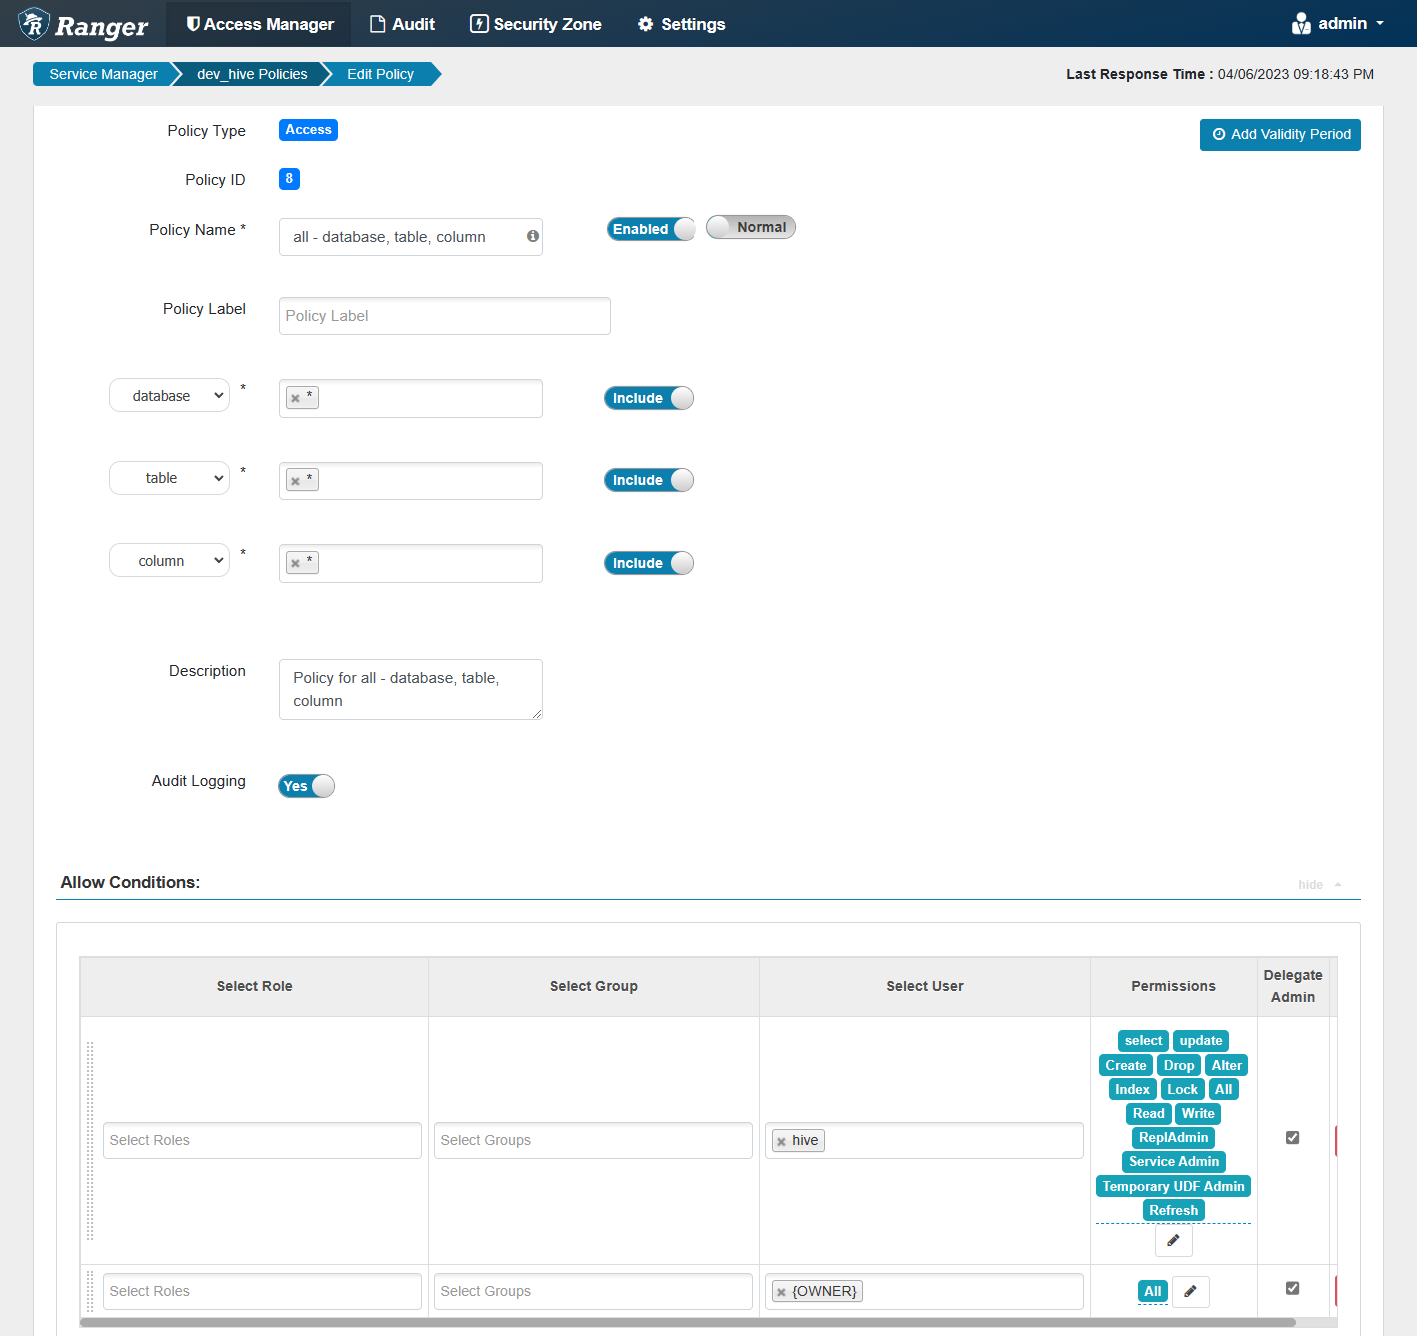
\includegraphics[width=0.65\textwidth]{chapters/tech_background/figures/ranger_hive_poly.png}}
    \caption{Sample configuration for a Hive service in Apache Ranger.}
    \label{fig:ranger_hive_details}
\end{figure}

\subsection{\label{sec:plugins_for_apache_ranger} Plugins for Apache Ranger}

All services defined in Apache Ranger are treated as plugins, sharing a common interface independent of what the external Service is doing. A plugin has two components:

\begin{itemize}
    \item \textbf{A service type definition} - also referred to as the \mintinline{text}{serviceDef.json} file. The file can be added as part of the source code in the folder \mintinline[breaklines, breakafter=/]{java}{agents-common/src/main/java/resource/service-defs} and loaded in the service definition repository in the class \mintinline{text}{EmbeddedServiceDefsUtil}, or updated dynamically using a POST request to \mintinline[breaklines, breakafter=/]{text}{/public/v2/api/servicedef}.
    \item \textbf{A serivce implementation} - a class that extends the abstract class \mintinline{java}{RangerBaseService}.
\end{itemize}

The properties defined by the service type definition JSON of most relevance are the id, name, implementation class name, a list of resource types, access types and configuration properties.

Apache Ranger defines access types by an id, a name and their implied grants (a list of names of other access types defined in the same file) and specifies how a user can interact with a resource, being the lowest level granularity for access control. Access types use implied grants to create an alias for a set of access types, where the parent access type is allowed for a resource if and only if all the child access types are allowed for that resource. These aliases can be recursive. Common access types are: \mintinline{java}{Create}, \mintinline{java}{View}, \mintinline{java}{Edit} and \mintinline{java}{Delete}. The service type definition specifies all possible access types and each resource selects which access types apply to it.

Apache Ranger defines resource types by an id, a name, a type (\mintinline{java}{string}, \mintinline{java}{path} or \mintinline{java}{url}), a parent (the name of another resource type defined in the same file), their access type restrictions (a list of names of access types from the same file), a level, and a mandatory flag, among other which are beyond the scope. The parent property is fundamental and used to create resource hierarchies. Apache Ranger structures resources as a graph, which can be conceptualised as a tree (a connected acyclic undirected graph) where the root node holds no data and all its immediate children are resources with no parent. The path from the root to the node representing that resource fully-quantifies the resource. For example, take a database system that structures data in databases, tables and columns; the database name is globally unique, but the table and column names are; thus, to fully specify a column, the table containing it and the database includes that table is needed. Access type restrictions are the mechanism used by resource types to determine which access types apply to them.

Configuration properties define inputs needed when creating a new service instance to connect to the external service.

The service implementation class, extending \mintinline{java}{RangerBaseService} must implement two function:

\begin{itemize}
    \item \mintinline{java}{public Map<String, Object> validateConfig();} Validates the configuration properties passed to the creation of a new service instance. The configuration is passed to the class's constructor, so the function takes no parameters. The function needs to return a map with specific key-value pairs, generated with the \mintinline{java}{BaseClient.generateResponseData}, or throw a \mintinline{java}{HadoopException} if validation fails. It is common for this function to verify connection to the external service, but this is not a requirement.
    \item \mintinline[breaklines]{java}{public List<String> lookupResource(ResourceLookupContext context) throws Exception;} Handle the auto-complete functionality used by the user interface by querying the external resource for resource names that match a prefix and a context.  
\end{itemize}

The abstract base class has other functions that can be overridden but are not covered here. 

It is essential to make clear that the Ranger Security Admin Service uses the service implementation class for quality-of-life features, such as resource name autocompletes and default policy generation, but is not utilised by mechanisms that handle access control and policy evaluation. Apache Ranger provides a default implementation of the abstract class, \mintinline{java}{RangerDefaultService}, which implements both abstract functions to return empty responses and enable the creation of new service types dynamically, with no changes to the source or redeployment of the Security Admin Service needed.

\subsection{Plugins for External Services}

For all external services that use Apache Ranger for authorisation\footnote{This report uses a mix of the British English "to authorise" and the American English "to authorize". We use the British English form in normal writing and the American English form for component and class names. This is done to comply with OpenMetadata and Apache Ranger coding standards.}, evaluation of policies is done on the application side, using libraries provided by Apache Ranger, not on the Security Admin Service side.

The implementation of plugins for external services usually is comprised of the implementation of the authorisation interfaces provided by the service (e.g., \mintinline{java}{HiveAuthorizerFactory} and \mintinline{java}{AbstractHiveAuthorizer} for Hive) and adjacent utility classes. These implementations are not used directly but rather through shim classes. A shim is a library that intercepts API calls, altering their functionality, usually used to support compatibility between versions and to run programs in non-native environments \cite{shimsNewton2011}. In this case, shims handle compatibility between Apache Ranger libraries, which are compiled for Java 8 and have dependencies on deprecated JavaEE libraries, and the external service's libraries so all can run as part of the same Java program.

Apache Ranger provides three packages used by plugins in external services:

\begin{itemize}
    \item \mintinline{java}{org.apahce.ranger:ranger-plugins-common} - Logic for policy evaluation;
    \item \mintinline{java}{org.apache.ranger:ranger-plugins-audit} - Audit management system that handles local collection and batching of audit logs and offloading to the Audit Store;
    \item \mintinline{java}{org.apache.ranger:ranger-plugin-classloader} - Specialised child-first class loader used by shim classes.
\end{itemize}

\subsection{Local development and debugging}

The Security Admin Service is a Spring application running on an embedded Tomcat server, which heavily uses dynamic loading of classes for plugins, so running and debugging this setup for local development is complex. This section proposes a process for running the Apache Ranger system locally, attaching a debugger and reloading the Security Admin Service with new changes.

We will extensively use the Docker Compose harness provided by Apache Ranger to run the core system and external services, as documented by the \mintinline{text}{dev-support/ranger-docker/README.md} file.

Software requirements are a Java Development Kit installation version 11, Apache Maven, Docker and Docker Compose. 

A prerequisite step is upgrading the Docker Compose harness to run on Java 11 instead of Java 8, which is required for the integration with OpenMetadata, which is covered in later chapters. The upgrade consists of two changes:

\begin{itemize}
    \item The \mintinline{text}{dev-support/ranger-docker/Docker.ranger-base} Docker file uses OpenJDK version \mintinline{text}{openjdk-8-jdk}, which should be updated to \mintinline{text}{openjdk-11-jdk};
    \item The \mintinline{text}{embeddedwebserver/scripts/ranger-admin-services.sh} script that starts the Security Admin Service uses Java options \mintinline[breaklines, breakafter=/-:]{java}{-Xloggc:{XAPOLICYMGR_EWS_DIR}/logs/gc-worker.log -verbose:gc -XX:+PrintGCDetails}, controlling logs from the garbage collector, which are deprecated in Java 11 and should be removed.
\end{itemize}

The continuous development setup requires two steps to initialize the environment that does not need to be repeated for future changes:

\begin{enumerate}

\item A full, successfully terminating build of the Apache Ranger project that will create all the Java artefacts;
\begin{minted}{bash}
mvn clean compile package install -DskipTests -DskipJSTests
\end{minted}

\item A complete, successful run of the flow described by \mintinline{text}{dev-support/ranger-docker/README.md}, following point \textit{5.ii} and skipping point \textit{5.i} to build Docker images.

\end{enumerate}

Let \mintinline{java}{<module>} represent the module with source code changes that need to be integrated into the Docker Compose harness. Listing \ref{listing:ranger_module_reload_bash} provides the source code for a bash script that implements the procedure to update the running Security Admin Service with new changes. Lines 3 and 4 handle building the module classes and the Security Admin Service artefact, respectively. Lines 8 to 10 handle building a new Docker image based on the new build artefact, removing the old container and recreating it with the new image. 

\begin{listing}
\centering
\begin{minted}[breaklines,linenos]{bash}
!#/bin/bash
set -x
mvn clean compile package install -DskipTests -DskipJSTests -Dpmd.skip -pl :<module>
mvn package -DskipTests -DskipJsTests -Dpmd.skip -P -all,-ranger-jdk11,ranger-admin -rf :ranger-distro
rm -rf dev-support/ranger-docker/dist/ranger-*-admin.tar.gz
cp target/ranger-*-admin.tar.gz dev-support/ranger-docker/dist
cd dev-support/ranger-docker
docker-compose -f docker-compose.ranger.yaml build --no-cache
docker-compose -f docker-compose.ranger.yml -f docker-compose.ranger-postgres.yml kill ranger
docker-compose -f docker-compose.ranger.yml -f docker-compose.ranger-postgres.yml up -d --no-deps ranger
\end{minted}
\caption{\label{listing:ranger_module_reload_bash} Bash script for reloading Apache Ranger's Docker Compose local setup to include source code changes from a module.}
\end{listing}

\section{OpenMetadata}

The OpenMetadata system is written in multiple languages (Java, Python and Typescript); its source code is packaged as an Apache Maven project with submodules representing different parts of the framework. The system is composed of the following elements:

\begin{itemize}
    \item \textbf{Metadata Store} - PostgreSQL or MySQL database that stores metadata information;
    \item \textbf{Search Engine} - Elasticsearch engine for fast queries of metadata information;
    \item \textbf{Standard Schemas} - definitions for types and entities used across all the components, defined using JSON Schemas (module \mintinline{text}{org.open-metadata:openmetadata-spec});  
    \item \textbf{Metadata Service} - web service, written in Java, based on the Dropwizard framework, that governs access to metadata and provides the system's API (module \mintinline[breaklines,breakafter=.:-]{java}{org.open-metadata:openmetadata-service});
    \item \textbf{User Interface} - single page application, written Typescript, using the React framework (module \mintinline{text}{org.open-metadata:openmetadata-ui});
    \item \textbf{Ingestion Framework} - Python package that crawls data stores to gather and report metadata (PiPy package \mintinline{text}{openmetadata-ingestion}).
\end{itemize}

Figure \ref{fig:openmetadata_arch} represents a compact architectural diagram of the OpenMetadata system. Components marked with dotted lines represent external services. 

\begin{figure}
    \centering
    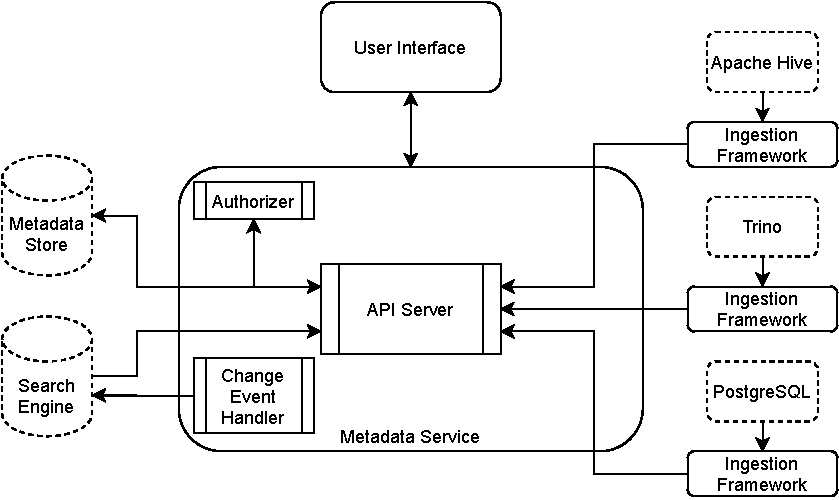
\includegraphics[width=0.8\textwidth]{chapters/tech_background/figures/openmetadata-arch.pdf}
    \caption{Architectural diagram of the OpenMetadata system.}
    \label{fig:openmetadata_arch}
\end{figure}

\subsection{User Interface}

\begin{figure}
    \centering
    
    \subfloat[\centering \label{fig:openmetadata_sample_data_table} Page showing metadata of a sample table in OpenMetadata.]{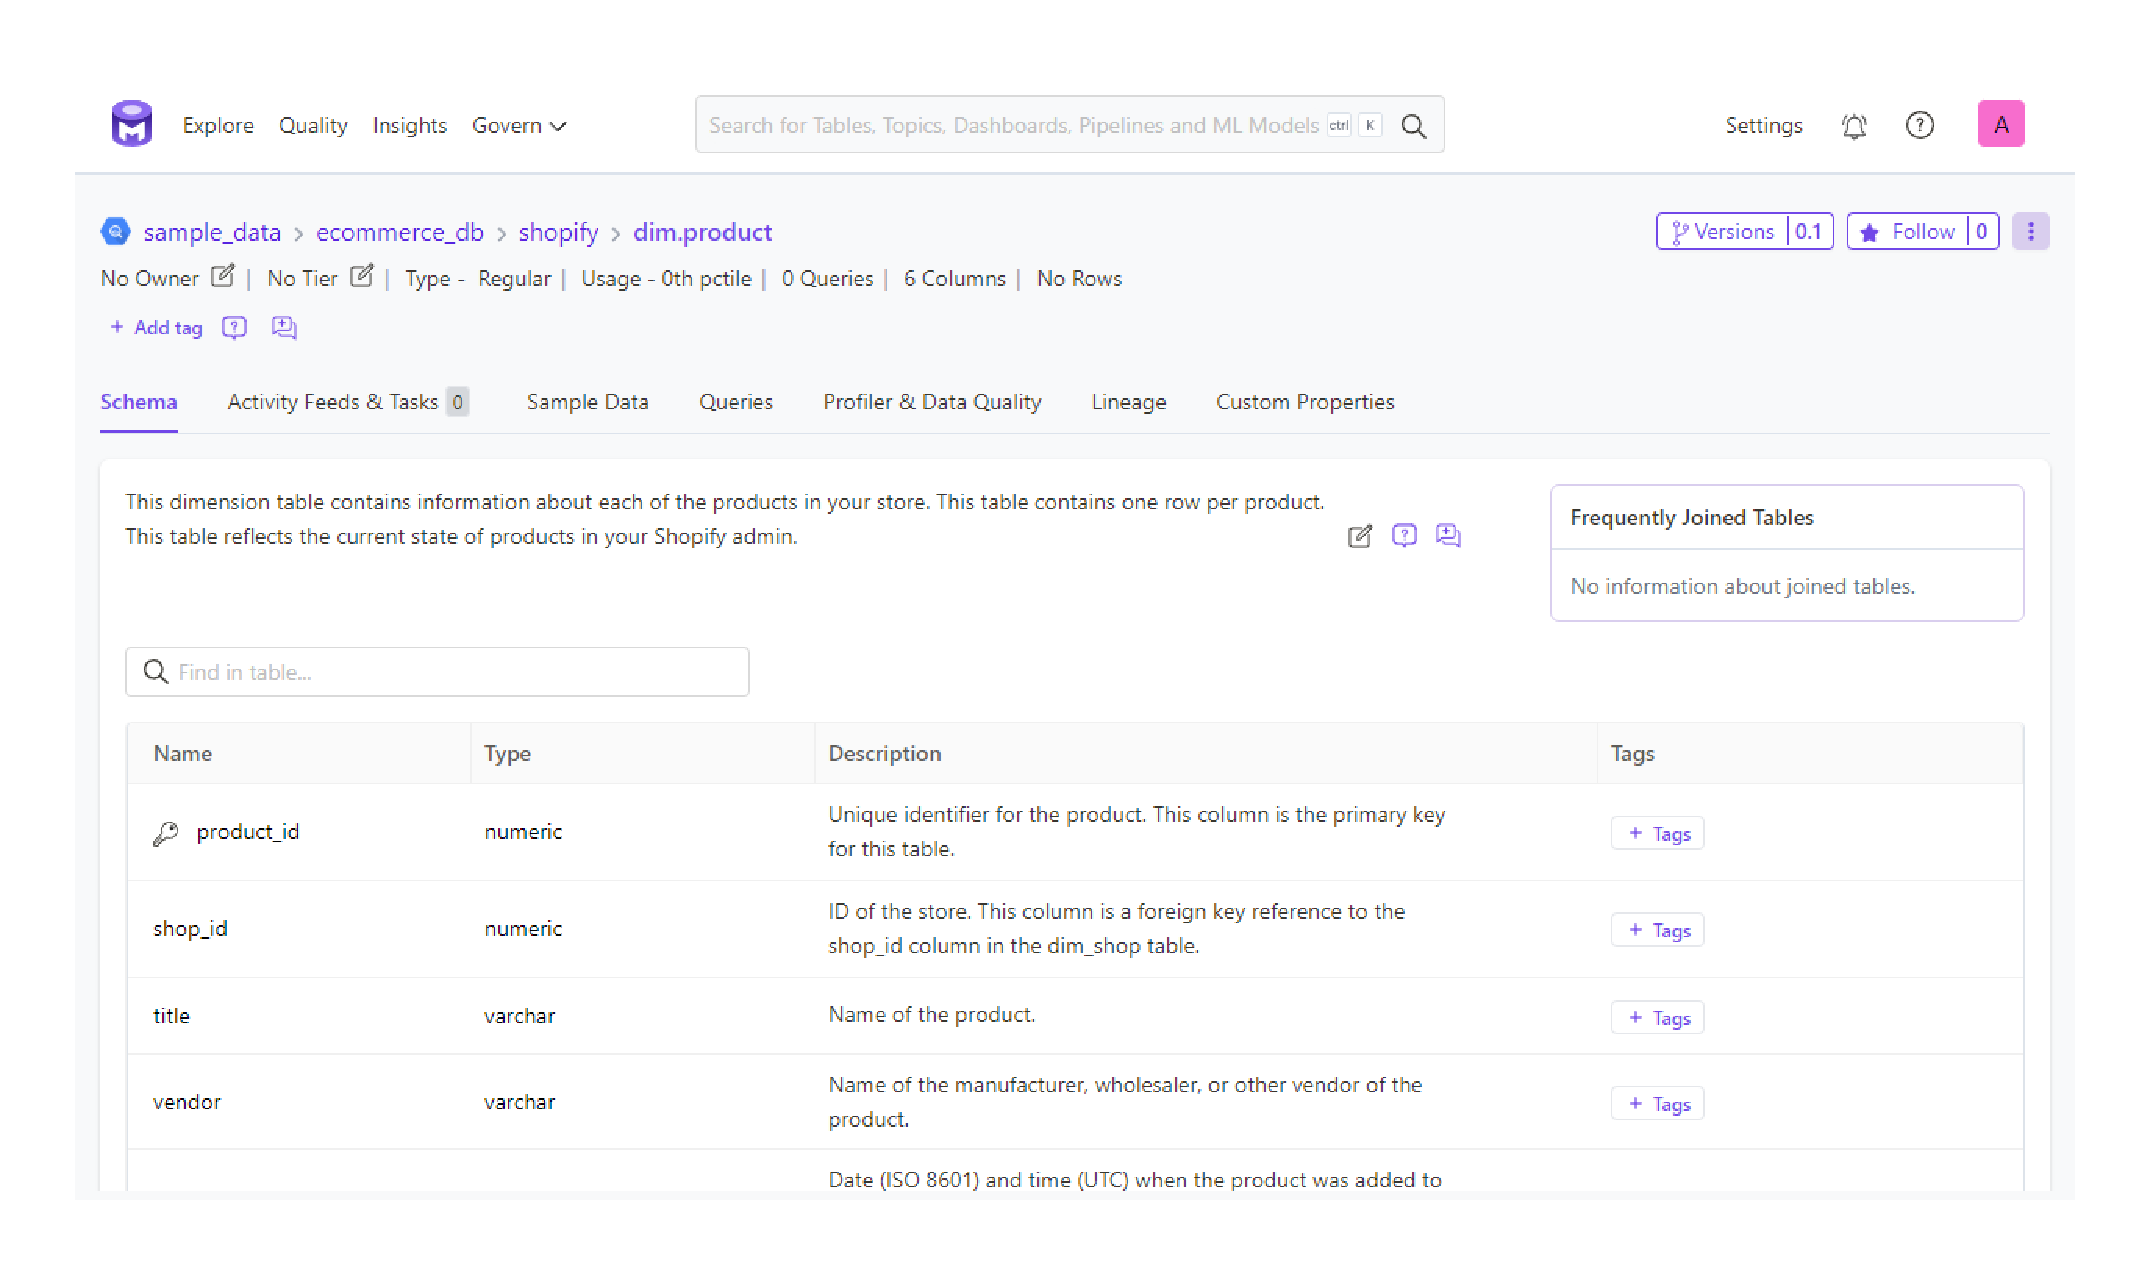
\includegraphics[width=0.8\textwidth]{chapters/tech_background/figures/openmetadata_sample_data_table.pdf}} 

    \qquad

    \subfloat[\centering \label{fig:openmetadata_sample_data_explore} Search page from OpenMetadata.]{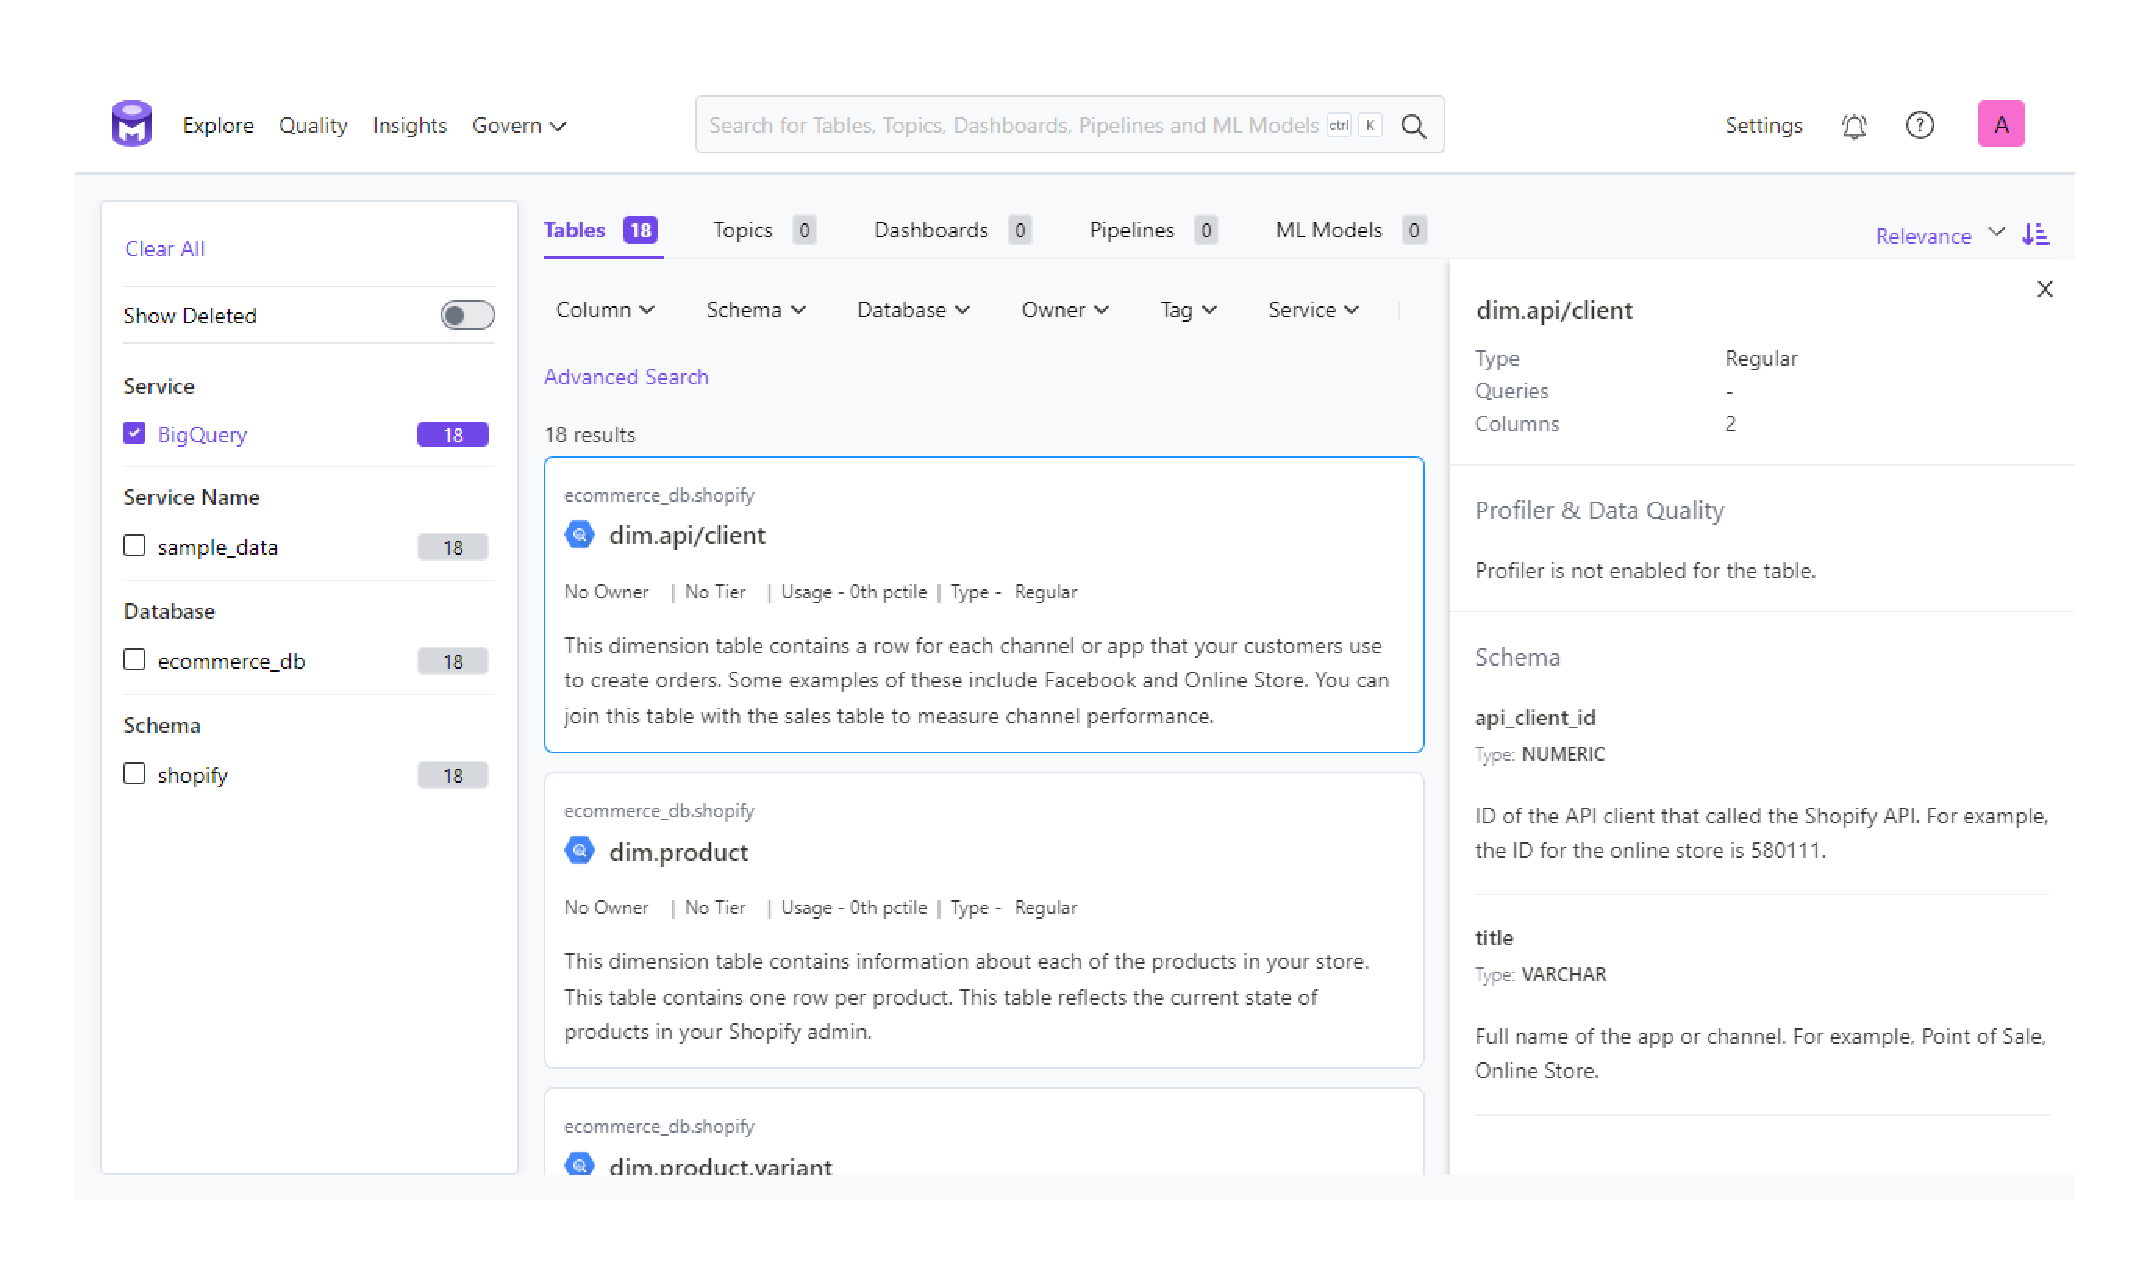
\includegraphics[width=0.8\textwidth]{chapters/tech_background/figures/openmetadata_sample_data_explore.pdf}}
    
    \caption{Sample screenshots from the OpenMetadata user interface.}
\end{figure}

The user interface is how data analysts, data scientists and domain experts interact with the OpenMetadata system to search for resources, view metadata, edit descriptions, tag datasets, and collaborate.

Figure \ref{fig:openmetadata_sample_data_table} shows the information page of the \mintinline{text}{shopify>dim.product} tables ingested from a Google Big Query database, containing the fully quantified name of the resource, the schema of the table, the type of each column, description, owner information and associated tags, among others. This page also provides functionality for editing user-modifiable metadata about the resource, like the description and tags.

Figure \ref{fig:openmetadata_sample_data_explore} shows the system's search functionality. The left-hand side panel contains facet-style filters used to remove unwanted results quickly. The right-hand side panel has a preview of the selected resource. The central panel lists all the results of the search along with more filters for specific properties of tables and a complex query builder under the "Advanced Search" button.

Functionally, the user interface uses the publicly exposed APIs of the Metadata Service and an authentication provider to handle logins. The build process dynamically generates Typescript interfaces from the Standard Schemas provided as JSON schemas which are then available in the user interface source code.

\subsection{Metadata Service}

The Metadata Service is the system's core, governing all reading, updating, creating and deleting metadata. The system treats all resources (e.g., databases, tables, tags, users, dashboards, workflows) as entities, sharing a common interface, defined in the Standard Schema as \mintinline{java}{EntityInterface}. The \mintinline{java}{EntityReference} type provides links to other entities without storing their full representation. Entities can have extensions, storing additional information that can optionally be fetched if needed, and two entities can have a relationship, which can further store information about their relationship.

The API provides a common pattern of endpoints for CRUD operations on all entity types, and certain entities also support specialized operations. We list examples of common requests below:

\begin{itemize}
    \item \mintinline{text}{GET /api/v1/<entityType>/<id>} - retrieves an Entity instance by ID;
    \item \mintinline{text}{GET /api/v1/<entityType>/name/<fullyQualifiedName>} - retrieves an Entity instance using its fully qualified name;
    \item \mintinline{text}{PUT /api/v1/<entityType>} - updates an existing Entity instance or creates a new one.
\end{itemize}

\subsection{Access Control Mechanism}

The Metadata Service handles access control for all operations that interact with entities through an \mintinline{java}{Authorizer} interface, which checks the subject's permission to apply an action to a resource. The included implementation of this interface (aptly named \mintinline{java}{DefaultAuthorizer}) uses a role-based access control system established on the NIST "Flat RBAC" model \cite{nistRBAC2000Sandhu, buildingAccessControlForOpenMetadata2022Mathew}, which is very similar to the mechanism employed by Apache Ranger, with some essential differences that will be discussed later. 

The model defines the following components:

\begin{itemize}
    \item \textbf{Rules} - an object comprised of a set of resource types, a set of access types, an effect, which can be either allowed or denied, and a condition, written in the Spring Expression Language (SpEL);
    \item \textbf{Policy} - a set of rules;
    \item \textbf{Role} - a set of policies where each policy can be enabled or disabled.
\end{itemize}

Users are assigned roles case-by-case or through their teams and departments. The user interface handles all configuration, and the Metadata Store stores the rules, policies and roles. Conditional rules enable contextual matching, affecting only resources which meet criteria (e.g., the \mintinline{java}{isOwner()} directive matches only resources of which the current user is the owner). 

\subsection{Downfalls of the included authorization system and the need for Apache Ranger}

The access control system included with OpenMetadata was designed to provide an adequate solution for small to medium-sized organizations, where migrating users and departments to OpenMetadata is manageable with no automation and the level of access granularity need not be too precise.

We claim that the provided system is inadequate for large organizations, with particular attention to organizations that implement company-wide access control systems looking for precise access control of their metadata and wish to integrate OpenMetadata with existing infrastructure.

\begin{enumerate}

    \item \textbf{Granularity of resources in rules.} Access control rules can be applied to all resources of a particular type but not to specific resources; thus, constraining access on a resource-by-resource basis is impossible. For example, a rule can allow reading of all table resources, but not specifically of the \mintinline{text}{sample_data>ecommerce_db>shopify>dim.product} table. Condition rules mimic this behaviour but are limited and challenging to manage and, thus, not a suitable alternative.

    \item \textbf{Integration with Active Directory.} Active Directory systems are, for many organizations, the central database of users and groups and often serve as a common language for integrating with proprietary or legacy software; thus, they need to be a part of the access control framework. OpenMetadata could adapt to these systems by mimicking a subset of the resource structures in an Active Directory employing its internal representation of users and teams. Still, this process is not officially supported and is likely prone to desynchronization issues.

    \item \textbf{Governance of access control and administration.} Finally, the security of such a system is only as good as the access control rules that govern it. OpenMetadata manages these through the UI and handles permissions to view or modify rules and policies using the authorization system; thus, it suffers from the issues outlined in point 1.

\end{enumerate}

These deficiencies motivate integrating OpenMetadata with Apache Ranger, as the latter is an industry-tested tool that aims to tackle these issues.

\subsection{Conclusion}

This chapter has laid out the groundwork needed for the next chapter, which proposes a system design and an implementation. Further, it motivates issues with the current approach and why the solutions are required. Section \ref{sec:tech_background_apache_ranger} aims to stand alone as an introduction to the inner workings of Apache Ranger. At the same time, the following chapters provide a practical example of using Apache Ranger libraries to handle authorisation for other services.
    \chapter{Design}

This chapter covers the architectural design of the proposed system for integrating Apache Ranger as an access control system for OpenMetadata. It lays out the high-level structural components, details the protocol these use to communicate and outlines the approaches used. Comprehensive details of the implementation are covered in the next chapter.

\section{High-level architectural overview}

\begin{figure}
    \centering
    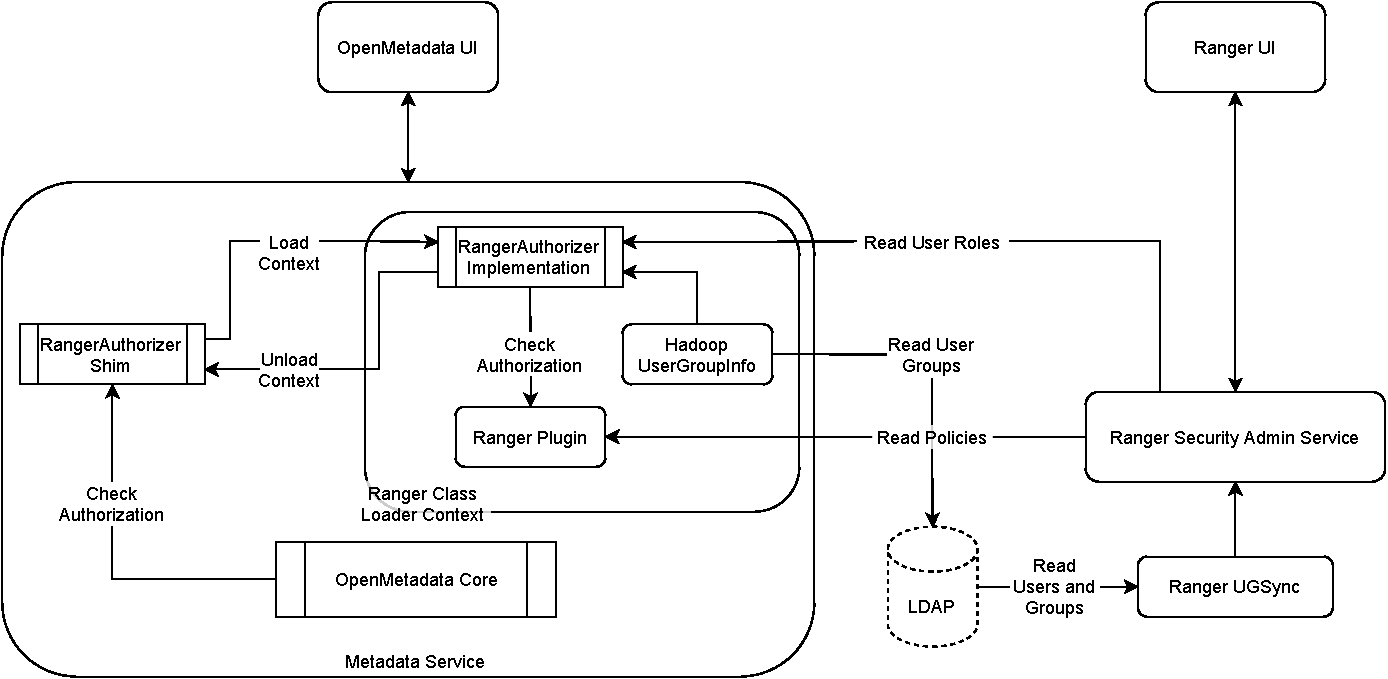
\includegraphics[width=0.8\textwidth]{chapters/design/figures/openmetadata-ranger-arch.pdf}
    \caption{High-level architectural overview of OpenMetadata and Apache Ranger system integration.}
    \label{fig:openmetadata-ranger-arch}
\end{figure}

\begin{figure}
    \centering
    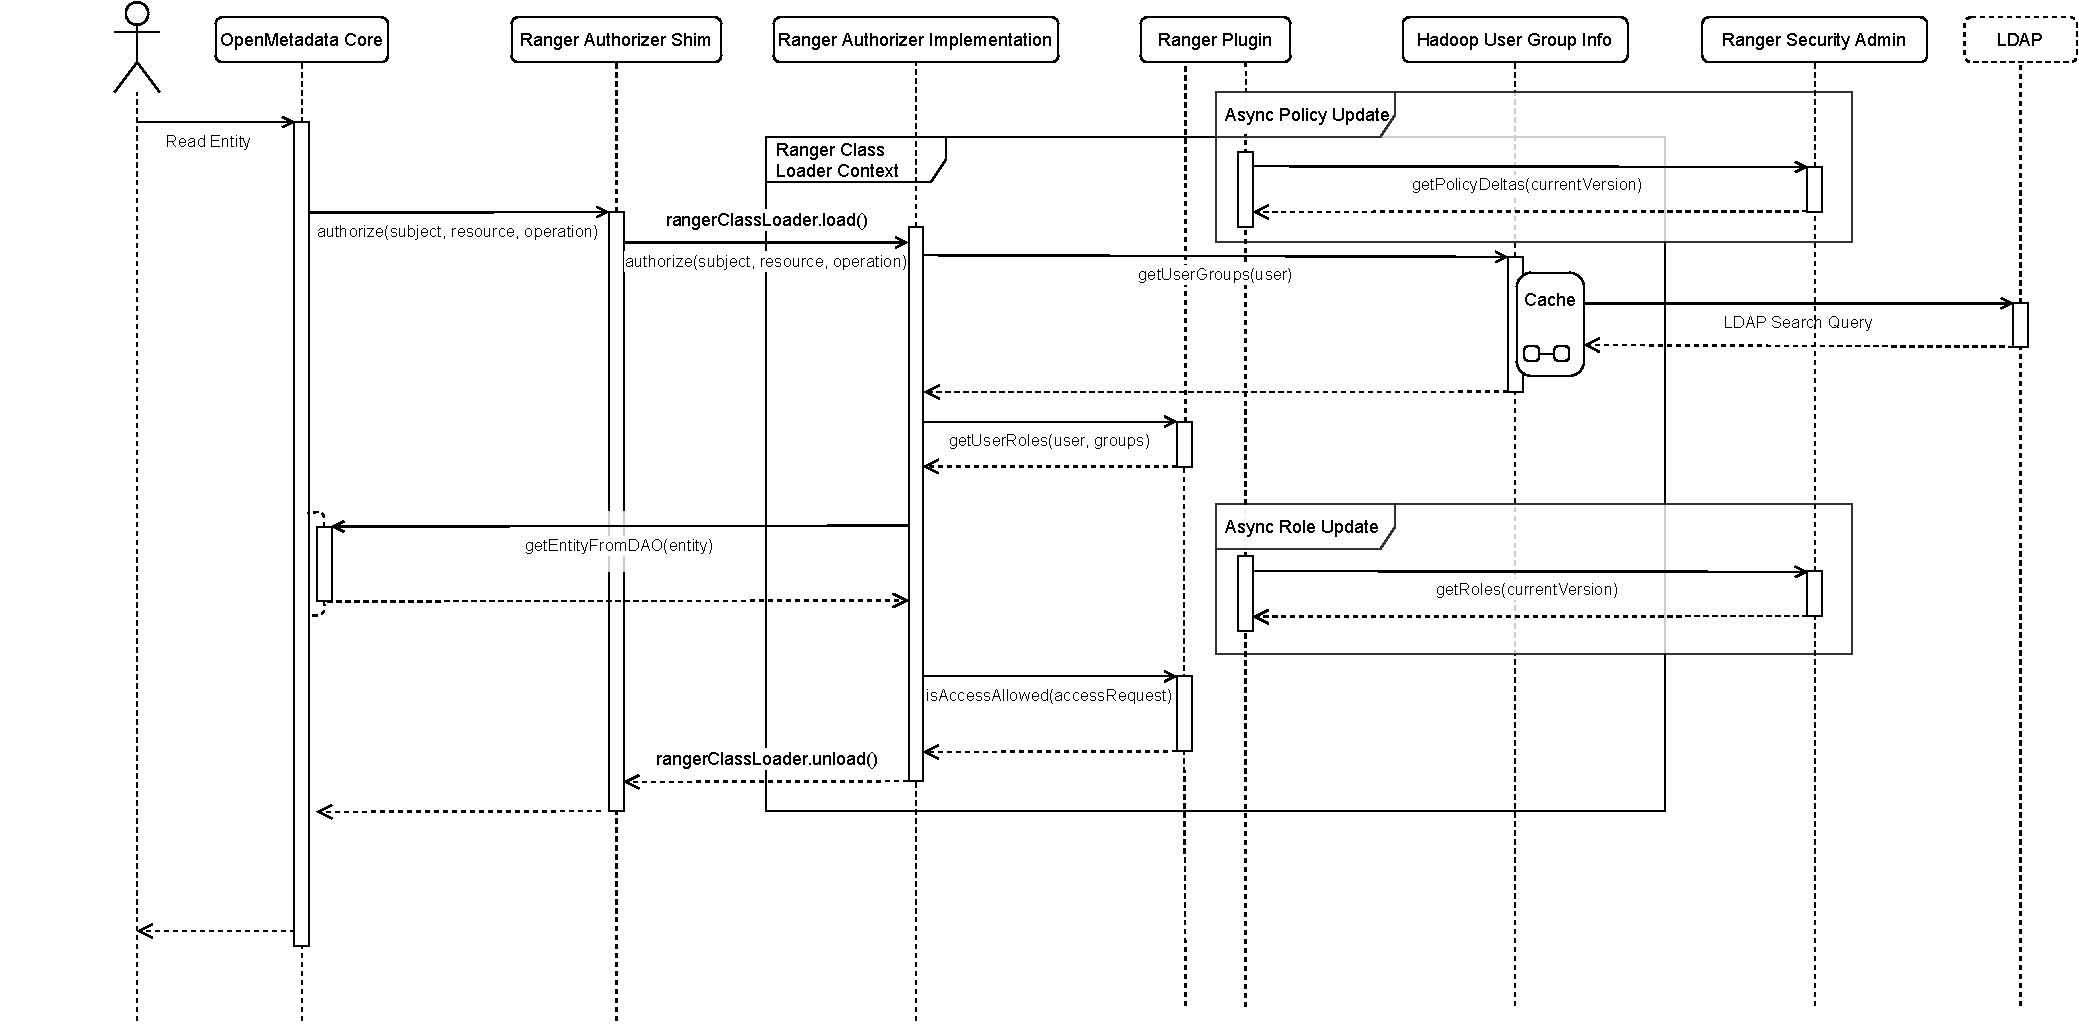
\includegraphics[width=\textwidth]{chapters/design/figures/openmetadata-ranger-lifecycle.pdf}
    \caption{High-level lifecycle of an  OpenMetadata authorisation request using Apache Ranger.}
    \label{fig:openmetadata-ranger-lifecycle}
\end{figure}

We begin by defining all the primary components of the system:

\begin{itemize}
    \item \textbf{OpenMetadata Core} - core OpenMetadata systems that handle loading entities from the Metadata Store, processing requests and calling the access control system when needed;
    \item \textbf{Ranger Authorizer Shim} - lightweight shim class that mediates calls to OpenMetadata's Ranger Authorizer Implementation by loading and unloading the class loader context;
    \item \textbf{Ranger Authorizer Implementation} - working components that use Apache Ranger libraries to handle authorization;
    \item \textbf{Hadoop User Group Information} - a configured instance of Hadoop libraries for reading a user's groups from an Active Directory or LDAP system;
    \item \textbf{Ranger Plugin} - a configured instance of the Apache Ranger policy evaluation libraries;
    \item \textbf{Ranger Security Admin Service}, \textbf{Ranger UGSync}, \textbf{LDAP} - same as previous definitions.
\end{itemize}

Figure \ref{fig:openmetadata-ranger-arch} illustrates the logical layout of components and how these communicate with each other. OpenMetadata Core is the entry point into the system and initialises authorisation requests. Ranger UGSync is complement asynchronous, running on an internal timer independent of events in the system. The OpenMetadata Core, Ranger Auhorizer Shim, Ranger Authozier Implementation, Hadoop User Group Information libraries and Ranger Plugin libraries are part of the same Java process, namely the Metadata Service. Still, the latter three are isolated in a Java class loader context that is unavailable to other components and is only accessible through the shim class.

Figure \ref{fig:openmetadata-ranger-lifecycle} represents the authorisation lifecycle of a read request sent by a user (directly through the API or through the UI) to OpenMetadata and how the various components communicate. The time axis (the vertical axis) is not to scale. 

OpenMetadata Core initiates an authorisation request by calling the Shim class, which loads the Ranger Class Loader Context and passes the call to the Ranger Authorizer Implementation. Evaluating the authorisation request has four steps: querying user groups from the Hadoop User Group Info provider, getting the roles based on the user and groups from the Ranger Plugin, loading the entity data from OpenMetadata Core (if not already provided) and finally, using the Ranger Plugin to check access. Once access has been decided, it returns and gives control to the Shim, which unloads the Ranger Class Loader Context and returns to the Core.

Hadoop User Group Info hits LDAP, the centralised user and groups database, and uses an in-memory cache to store results. Ranger Plugin keeps in-memory records of the policies and roles, asynchronously querying the Ranger Security Admin Service to update these.

This architecture combines synchronous and asynchronous operations and expensively uses in-memory duplication of remote resources to improve performance and avoid, as much as possible, calling external services in the critical path of access control evaluation.

\section{Service definition for OpenMetadata service types in Apache Ranger}

As discussed in Section \ref{sec:plugins_for_apache_ranger}, Apache Ranger requires a definition of the structure of OpenMetadata services, its resource types, access types, configuration properties and the implementation class. 

% We now focus on the resource types tree and access types.

OpenMetadata already defines internal resource names and access types the included access control system uses in the \mintinline[breaklines, breakbefore=/]{java}{openmetadata-serivce/src/main/resources/json.data/ResourceDescriptors.json} file found in the source code. The Apache Ranger service definition will follow the same naming scheme and implement a similar structure to maintain consistency. OpenMetadata resource names use camel casing (e.g., \mintinline{text}{databaseService}), which is not supported by Apache Ranger resource names as these do not accept capital letters, so a conversion to underscore case is applied (e.g., \mintinline{text}{database_service}).

The complete service definition for OpenMetadata services in Apache Ranger is provided in Appendix \ref{cha:servicedef_full}. It is also available in the \mintinline[breaklines, breakbefore=/]{java}{agent-common/src/main/resources/service-defs/ranger-servicedef-openmetadata.json} file in the Apache Ranger source code.

\subsection{Resource Types}

The resource tree is built using the resource types defined by OpenMetadata. A virtual root node that holds no that is used. One-to-many relationships between parent and child resource types give the hierarchy. Listing \ref{listing:tree_openmetadata_resources} provides a graphical representation of the resource tree.

OpenMetadata does not currently use the Feed resource type, but it is included here for forwards-compatibility. Tag and Glossary Term resources are recursive.

\begin{listing}
    
    \renewcommand\DTstyle{\rmfamily}
    \dirtree{%
    .1 Root. 
    .2 Database Service \DTcomment{\mintinline{text}{databaseService}}.
    .3 Database \DTcomment{\mintinline{text}{database}}.
    .4 Database Schema \DTcomment{\mintinline{text}{databaseSchema}}.
    .5 Table \DTcomment{\mintinline{text}{table}}.
    .2 Dashboard Service \DTcomment{\mintinline{text}{dashboardService}}.
    .3 Dashboard \DTcomment{\mintinline{text}{dashboard}}.
    .3 Chart \DTcomment{\mintinline{text}{chart}}.
    .2 Messaging Service \DTcomment{\mintinline{text}{messagingService}}.
    .3 Topic \DTcomment{\mintinline{text}{topic}}.
    .2 Machine Learning Service \DTcomment{\mintinline{text}{mlService}}.
    .3 Machine Learning Model \DTcomment{\mintinline{text}{mlModel}}.
    .2 Pipeline Service \DTcomment{\mintinline{text}{pipelineService}}.
    .3 Pipeline \DTcomment{\mintinline{text}{pipeline}}.
    .2 Storage Service \DTcomment{\mintinline{text}{storageService}}.
    .3 File Location \DTcomment{\mintinline{text}{location}}.
    .2 Metadata Service \DTcomment{\mintinline{text}{metadataService}}.
    .2 Glossary \DTcomment{\mintinline{text}{glossary}}.
    .3 Glossary Term \DTcomment{\mintinline{text}{glossaryTerm}}.
    .4 Glossary Term.
    .5 $\vdots$.
    .2 Tag Category \DTcomment{\mintinline{text}{tagCategory}}.
    .3 Tag \DTcomment{\mintinline{text}{tag}}.
    .4 Tag.
    .5 $\vdots$.
    .2 Bot \DTcomment{\mintinline{text}{bot}}.
    .2 Ingestion Pipeline \DTcomment{\mintinline{text}{ingestionPipeline}}.
    .2 User \DTcomment{\mintinline{text}{user}}.
    .2 Tams \DTcomment{\mintinline{text}{team}}.
    .2 Events \DTcomment{\mintinline{text}{events}}.
    .2 Feed \DTcomment{\mintinline{text}{feed}}.
    .2 Webhook \DTcomment{\mintinline{text}{webhook}}.
    .2 Custom Type \DTcomment{\mintinline{text}{type}}.
    .2 Test Suite \DTcomment{\mintinline{text}{testSuite}}.
    .3 Test Case \DTcomment{\mintinline{text}{testCase}}.
    .2 Web Analytic Event \DTcomment{\mintinline{text}{webAnalyticEvent}}.
    .2 Web Insight Chart \DTcomment{\mintinline{text}{webInsightChart}}.
    .3 KPI \DTcomment{\mintinline{text}{kpi}}.
    .2 Alert \DTcomment{\mintinline{text}{alert}}.
    .2 Alert Action \DTcomment{\mintinline{text}{alertAction}}.
    }

    \caption{Tree representation of OpenMetadata resource types.}
    \label{listing:tree_openmetadata_resources}
    
\end{listing}

\subsection{Access Types}

Access types define the operations that can be applied to resources. OpenMetadata utilises specialised access types to provide more precise access control for specific functions; e.g., the EditUsers access type enables adding or removing team members. 

Listing \ref{listing:tree_openmetadata_access_types} provides a graphical representation of the access types in OpenMetadata. The ViewAll and EditAll access types are shorthand for all view and edit operations. Unlike the tree of resource types, in the case of access types, a parent-child relationship does not imply ownership; thus, access types can be used independently of their parents.

Access types are not universally applicable to all resources type; each resource type specifies which access types can be used on it, e.g., Team resources support Create, Delete, ViewAll, EditAll, EditDisplayName, EditCustomFields and EditUsers operations. In contrast, Tables resources support all operations except EditUsers and EditStatus.

\begin{listing}

    \renewcommand\DTstyle{\rmfamily}
    \dirtree{%
    .1 All.
    .2 Create.
    .2 Delete.
    .2 ViewAll.
    .2 ViewBasic.
    .3 ViewUsage.
    .3 ViewTests.
    .3 ViewQueries.
    .3 ViewDataProfile.
    .3 ViewSampleData.
    .2 EditAll.
    .3 EditDescription.
    .3 EditDisplayName.
    .3 EditTags.
    .3 EditOwner.
    .3 EditTier.
    .3 EditCustomFields.
    .3 EditLineage.
    .3 EditStatus.
    .3 EditReviewers.
    .3 EditTests.
    .3 EditQueries.
    .3 EditDataProfile.
    .3 EditSampleData.
    .3 EditUsers.
    }

    \caption{Tree representation of OpenMetadata access types.}
    \label{listing:tree_openmetadata_access_types}
    
\end{listing}
    \chapter{Implementation}

This chapter covers the detailed implementation of all components needed for integrating Apache Ranger as an access control system for OpenMetadata. We also present engineering problems that arose during the implementation process and their solutions.

\section{Relocating the OpenMetadata Authorizer interface and related classes}

We begin by investigating the current Authorizer interface used by OpenMetadata, shown in Listing \ref{listing:original_authorizer}. The functions \mintinline{java}{listPermissions} and \mintinline{java}{getPermission} are used to query the operations a user is allowed to apply on all resource types, all resources under a specific resource type or a fully-qualified resource. The \mintinline{java}{authorize} function handles access control decisions, yielding successfully when access is authorised and throwing an \mintinline{java}{AuthorizerException} when it is not. The \mintinline{java}{authorizeAdmin} directive verifies that a user is an administrator of the system, throwing an exception otherwise. The final procedure, \mintinline{java}{decryptSecret}, is the process of being deprecated. 

The interface, along with all classes and other interfaces used in its definition, is part of the \mintinline{text}{org.open-metadata:openmetadata-serivce} submodule and is tightly bound to OpenMetadata's API service implementation. This is an issue, as the Apache Ranger authoriser implementation needs to be isolated in a separate submodule that does not depend on \mintinline{java}{openmetadata-service}. The solution proposed here is to relocate the \mintinline{java}{Authorizer} interface, with related classes and interfaces, to a new submodule \mintinline{text}{org.open-metadata:openmetadata-authorization}; thus, the API service implementation submodule and Apache Ranger authoriser submodule may then depend on it.

We define that \mintinline{text}{org.open-metadata:openmetadata-authorization} submodule to depend on the \mintinline{text}{org.open-metadata:openmetadata-spec} module, providing entity definitions, and to contain four interfaces under the \mintinline{java}{org.openmetadata.security} package: \mintinline{java}{Authorizer}, \mintinline{java}{OperationContextInterface}, \mintinline{java}{ResourceContextInterface}, \mintinline{java}{SecurityContextInterface} and the \mintinline{java}{AuthorizationException} class. The \mintinline{java}{Authorizer} interface is updated to use the new interfaces.

\begin{listing}

\begin{minted}[breaklines,
    linenos,
    fontsize=\footnotesize,
    frame=single,
]{java}
public interface Authorizer {
    void init(OpenMetadataApplicationConfig openMetadataApplicationConfig, Jdbi jdbi);

    List<ResourcePermission> listPermissions(SecurityContext securityContext, String user);

    ResourcePermission getPermission(SecurityContext securityContext, String user, String resource);

    ResourcePermission getPermission(
        SecurityContext securityContext, String user, ResourceContextInterface resourceContext);

    void authorize(
        SecurityContext securityContext, OperationContext operationContext, ResourceContextInterface resourceContext)
        throws IOException;

    void authorizeAdmin(SecurityContext securityContext);

    boolean decryptSecret(SecurityContext securityContext);
}
\end{minted}

\caption{Original \mintinline{java}{org.openmetadata.service.security.Authorizer} interface in the OpenMetadata source code.}
\label{listing:original_authorizer}

\end{listing}

\subsection{Initialisation}

The \mintinline{java}{OpenMetadataApplicationConfig} and \mintinline{java}{Jdbi} classes are part of the \mintinline[breaklines, breakafter=.:]{java}{org.open-metadata:openmetadata-serivce} module can not be used in the authorisation interface.

OpenMetadata handles the initialisation of resources in the \mintinline{java}{OpenMetadataApplication} class. The authoriser instance is created based on the \mintinline{text}{authorizerConfiguration.className} property provided by the application configuration. The following expression handles class loading and instance creation, the configuration properties being passed later to the \mintinline{java}{init} function.

\begin{minted}[breaklines, breakbefore=.]{java}
    this.authorizer = Class.forName(authorizerConf.getClassName()).asSubclass(Authorizer.class).getConstructor().newInstance();
\end{minted}

The initialisation sequence is updated to use the class constructor that takes a single argument, an instance of \mintinline{java}{AuthorizerConfiguration}, and the \mintinline{java}{init} function is modified to take no arguments.

\begin{minted}[breaklines, breakbefore=.]{java}
    this.authorizer = Class.forName(authorizerConf.getClassName()).asSubclass(Authorizer.class).getConstructor(AuthorizerConfiguration.class).newInstance(authorizerConf);
\end{minted}

The provided authoriser implementations, \mintinline{java}{DefaultAuthorizer} and \mintinline{java}{NoopAuthorizer}, are updated to follow the revised structure. Listing \ref{listing:new_authorizer} provides the final layout of the authorisation interface that the Apache Ranger authoriser will implement.

\begin{listing}

\begin{minted}[breaklines,
    linenos,
    fontsize=\footnotesize,
    frame=single,
]{java}
public interface Authorizer {
    default void init() {}

    List<ResourcePermission> listPermissions(SecurityContextInterface securityContext, String user);

    ResourcePermission getPermission(SecurityContextInterface securityContext, String user, String resource);

    ResourcePermission getPermission(
        SecurityContextInterface securityContext, String user, ResourceContextInterface resourceContext);

    void authorize(
        SecurityContextInterface securityContext,
        OperationContextInterface operationContext,
        ResourceContextInterface resourceContext)
        throws IOException;

    void authorizeAdmin(SecurityContextInterface securityContext);

    boolean decryptSecret(SecurityContextInterface securityContext);
}
\end{minted}

\caption{Updated \mintinline{java}{org.openmetadata.service.Authorizer} interface in the OpenMetadata source code.}
\label{listing:new_authorizer}

\end{listing}

\section{Using Apache Ranger libraries for authorisation}

This section details the initialisation and utilisation of Apache Ranger libraries for access control policy evaluation through the \mintinline{java}{RangerBasePlugin} class. It also touches on using the Hadoop user group information utility to retrieve users' group membership data for a centralised Active Directory database.

\subsection{Initialisation of the Ranger Plugin}

The Ranger base plugin loads its configuration from XML files structured as lists of key and value string pairs. This behaviour is handled by the \mintinline{java}{RangerPluginConfig} class that extends the commonly used Hadoop class \mintinline{java}{Configuration}.

Apache Ranger's configuration loading utility expects properties to be provided in three files, \mintinline{text}{ranger-<serviceType>-audit.xml}, \mintinline{text}{ranger-<serviceType>-security.xml} and\\ \mintinline{text}{ranger-<serviceType>-policymgr-ssl.xml} (where \mintinline{text}{<serviceType>} is a placeholder for the type of the service that the plugin is being initialised for, in this case taking the value \mintinline{text}{openmetadata}), which it will attempt to read from the current directory. We extend this functionality by allowing administrators to specify alternative locations for these files in OpenMetadata's configuration. The Hadoop utility for querying user group information is initialised similarly. Sample configuration files are in the OpenMetadata source code under the \mintinline{text}{ranger/openmetadata-authorization-ranger/conf} folder.

\section{\label{sec:utilising_the_ranger_plugin} Utilising the Ranger Plugin}

The Ranger plugin evaluates access requests using the function \mintinline{java}{isAccessAllowed}, which takes a single argument, an instance of the \mintinline{java}{RangerAccessRequest} class which wraps identification of the user requesting access (consisting of the user's unique name and the groups and roles it is a member of), a description of the resource being accessed, and the operation applied to the resource. 

User identification is handled by the mintinline{java}{RangerHadoopUserGroupsRolesProvider} class. Resolving the need data begins with the \mintinline{java}{SecurityContextInterface}, which supplies the user's name. The Ranger Authorizer uses the Hadoop User Group Information utility to get the user's groups.

\begin{minted}[breaklines, breakbefore=.]{java}
Set<String> groups = UserGroupInformation.createRemoteUser(internalName).getGroupNames();
\end{minted}

The Ranger Plugin is then used to retrieve the appropriate roles based on the user's name and the groups.

\begin{minted}[breaklines, breakbefore=.]{java}
Set<String> roles = rangerPlugin.getRolesFromUserAndGroups(user, groups);
\end{minted}

The Ranger Plugin handles references to resources as a mapping between string keys, representing the resource type, and generic objects, representing the value of the resource type, through the \mintinline{java}{RangerAccessResourceImpl} class. The generic objects used for resource values are commonly strings or collections of strings. The \mintinline{java}{RangerOpenmetadataAccessResource} class extends \mintinline{java}{RangerAccessResourceImpl}, implementing the mapping of OpenMetadata entities to key-values pairs recognised by the Ranger Plugin. The class handles setting values for entities with parents by reflectively invoking methods that take certain entity types as arguments, as depicted in Listing \ref{listing:ranger_openmetadta_access_resource}.

Since these are recursive types, Tag and Glossary Term entities require specialised resource-value mapping. A Tag object does not provide a reference to its Tag Category or parent Tag; thus, we build the resource path of a Tag from its fully quantified name. OpenMetadata defines a language for the fully qualified names of entities, a dot-separated list of strings which may be in quotes if containing special characters, using ANTLR; fully qualified names are split into their components by parsers generated by ANTLR. The Tag Category and ancestor Tags of a Tag entity can thus be derived from the elements of its fully qualified name. A Glossary Term entity contains references to its Glossary and parent Term, but to retrieve the parent of the parent Glossary Term a database read is required; we avoid this inefficiency but adopting the same approach as with Tag entities. For both Tags and Terms, the ancestors' names are joined with the forward-slash symbol (/) to create path-like strings recognised by the Ranger Plugin.

\begin{listing}

\begin{minted}[breaklines,
    linenos,
    fontsize=\footnotesize,
    frame=single,
]{java}
public class RangerOpenmetadataAccessResource extends RangerAccessResourceImpl {
    public RangerOpenmetadataAccessResource(ResourceContextInterface resourceContextInterface) {
        ...
        EntityInterface entity = resourceContextInterface.getEntity();
        try {
            Method method = this.getClass().getDeclaredMethod("setSubValues", entity.getClass());
            method.invoke(this, entity);
        } 
        ...
    }
    
    private void setSubValues(Table table) {
        setValue(table.getService(), DatabaseService.class);
        setValue(table.getDatabase(), Database.class);
        setValue(table.getDatabaseSchema(), DatabaseSchema.class);
    }
    
    ...

    private void setValue(EntityReference entityReference, Class<? extends EntityInterface> clazz) {
        if (entityReference == null) {
            setValue(formatOpenMetadataClassNameToRangerResource(clazz), "*");
        } else {
            setValue(entityReference);
            }
    }

    private void setValue(EntityReference entityReference) {
        setValue(getRangerResourceName(entityReference), entityReference.getName());
    }
}
\end{minted}

\caption{Snippet of the \mintinline{java}{RangerOpenmetadataAccessResource}, using reflection to set Ranger Access Resource values from OpenMetadata entities.}

\label{listing:ranger_openmetadta_access_resource}

\end{listing}

The access type is passed to the Ranger Plugin as a string, retrieved from the \mintinline[breaklines, breakbefore=CI]{java}{OperationContextInterface}. As this interface provides a list of operations, each is checked independently.

Listing \ref{listing:ranger_authorizer_impl_authorize} supplies the body of the \mintinline{java}{authorise} function provided by the Ranger Authorizer implementation of the OpenMetadata \mintinline{java}{Authorizer} interface. The procedure uses the \mintinline{java}{RangerOpenmetadataAccessRequest} class, which extends the provided request class \mintinline[breaklines, breakbefore=ARI]{java}{RangerAccessRequestImpl}, adding convenience constructors. The \mintinline{java}{isAccessAllowed} procedure of the Ranger Plugin returns a \mintinline{java}{RangerAccessResult} object, which contains the final allowed or denied decision along with meta information of the policy evaluations.

\begin{listing}

\begin{minted}[breaklines,
    linenos,
    fontsize=\footnotesize,
    frame=single,
]{java}
public void authorise (
        SecurityContextInterface securityContext,
        OperationContextInterface operationContext,
        ResourceContextInterface resourceContext)
        throws IOException {
    RangerUserGroupsRoles ugr = groupsRolesProvider.getUserGroupsRoles(securityContext);
    RangerAccessResource accessResource = new RangerOpenmetadataAccessResource(resourceContext);
    for (MetadataOperation operation : operationContext.getOperations()) {
        RangerAccessRequest req = new RangerOpenmetadataAccessRequest(accessResource, operation, ugr);
        RangerAccessResult result = rangerPlugin.isAccessAllowed(req);
        if (result != null && !result.getIsAllowed()) {
            throw new AuthorizationException(String.format("[RangerAccessRequest=%s] Permission denied by Ranger: %s", req, result));
        }
    }
}
\end{minted}

\caption{Snippet of \mintinline{java}{RangerAuthorizerImpl}, displaying the implementation of the authorisation check.}
\label{listing:ranger_authorizer_impl_authorize}
    
\end{listing}

\subsection{Listing user permissions for resources}

The Ranger Plugin enables queries of access control rules (commonly abbreviated to ACLs) with the procedure \mintinline{java}{getResourceACLs}, which accepts a single argument, a \mintinline[breaklines, breakbefore=AR]{java}{RangerAccessRequest} object. Creating an access request is the same as detailed above. An additional case appears when querying permissions for all resources of a type, which is handled by mapping, in the \mintinline{java}{RangerAccessResourceImpl}, the resource type and its ancestor to wildcards (the asterisk symbol).

The \mintinline{java}{getResourceACLs} function returns a \mintinline{java}{RangerResourceACLs} object containing three maps of the type \mintinline{java}{Map<String, Map<String, AccessResult>>}, one for each of user, group and role access control rules. Keys of the outer map represent the name of a user, group or role, respectively, while keys of the inner map represent access type, and values of the inner map represent an access result, which can be allowed, denied or undetermined. This response is not aggregated, as it will contain results for all users, groups and roles present in policies that match the resource queried and outcomes for all access types, not only those applicable to the resource type used in the request. Results are consolidated by the \mintinline{java}{RangerPermissionsProvider} class, filtering groups and roles the user is not part of and access types which do not correspond to the resource type in question, and combines the remaining results. An access type is considered permitted if any of the user's groups for roles allow it or if the user is specifically allowed that access type.

\section{Additional changes to OpenMetadata}

This section details changes to OpenMetadata's metadata service and user interface to empower better compatibility with the Ranger authoriser's more precise access control mechanism. When considering these changes, supporting complete backward compatibility and maintaining the same behaviour for the included authoriser is critical.

\subsection{Listing of entities}

OpenMetadata's included authorisation system does not distinguish between entities with the same resource type; thus, listing entities of a kind (e.g., tables) is authorised by checking that the principal user is allowed to perform the ViewAll action on all resources of that type. This approach does not operate well with the more precise access control imposed by the Ranger authoriser, where a user may be allowed to view a subset of tables but not all.

The listing of entities paginates results, returning two pointers to the start and end of the list of results, which can be used by future requests to fetch the next or previous page of entities. As the access control evaluation is done inside the metadata service, it cannot be known if the user is allowed to view a resource before fetching it from the database; at the same time, it is ideal for reducing the number of entities unnecessarily retrieved from storage. The solution proposed fetches singular entities, checks access permission for the user on that resource and adds it to the page or discards it accordingly until the page is filled. This approach avoids the issue of retrieving too many entities so that the page is completed before all can be evaluated, thus wasting resources; it is a trade-off between the cost of a round-trip to the database and the cost of transporting and deserialising more data. 

\subsection{Masking results on the Search page}

OpenMetadata maintains a copy of the metadata in Elasticsearch, which is used for fast searches, input autocompletion and aggregations. Searching through entities is available with two API endpoints  \mintinline{text}{/api/v1/search/query} and \mintinline{text}{/api/v1/search/suggest}. These endpoints only enable the reading of some metadata entities but bypass the access control mechanisms; thus, metadata that the user is not privileged to view can appear in the search results. This is a known security issue of the platform, with plans to fix it in future versions. It is also a complex issue to resolve since the access control system may add too much overhead to the search functionality, diminishing one of its main primary purposes, fast resource lookup; additionally, since filtering of results from the search engine needs to be done by the metadata service, the values of total results, hit scoring and aggregations would be skewed. For these reasons, the issue of access control mechanism for search results in OpenMetadata is beyond the scope of this report.

We provide a mechanism for signalling to the users using the Search page in OpenMetadata's user interface that they are not privileged to view some of the entities presented. Recall Figure \ref{fig:openmetadata_sample_data_explore}, showing the Search page and the right-hand side panel, which appears when the user clicks on one of the search results. If the user is not allowed to view the entity (table in this case), the panel will not show any data, instead displaying a suitable message, as illustrated in Figure \ref{fig:openmetadata_sample_data_explore_denied}. The feature is implemented as part of the UI, calling the \mintinline{java}{/api/v1/permissions/{resource}/{id}} API endpoint to list the permissions of the current user on the given resource.

It is essential to highlight that this change does not improve the system's security, as data is still available programmatically - it is only an improvement to the user experience.

\begin{figure}
    \centering
    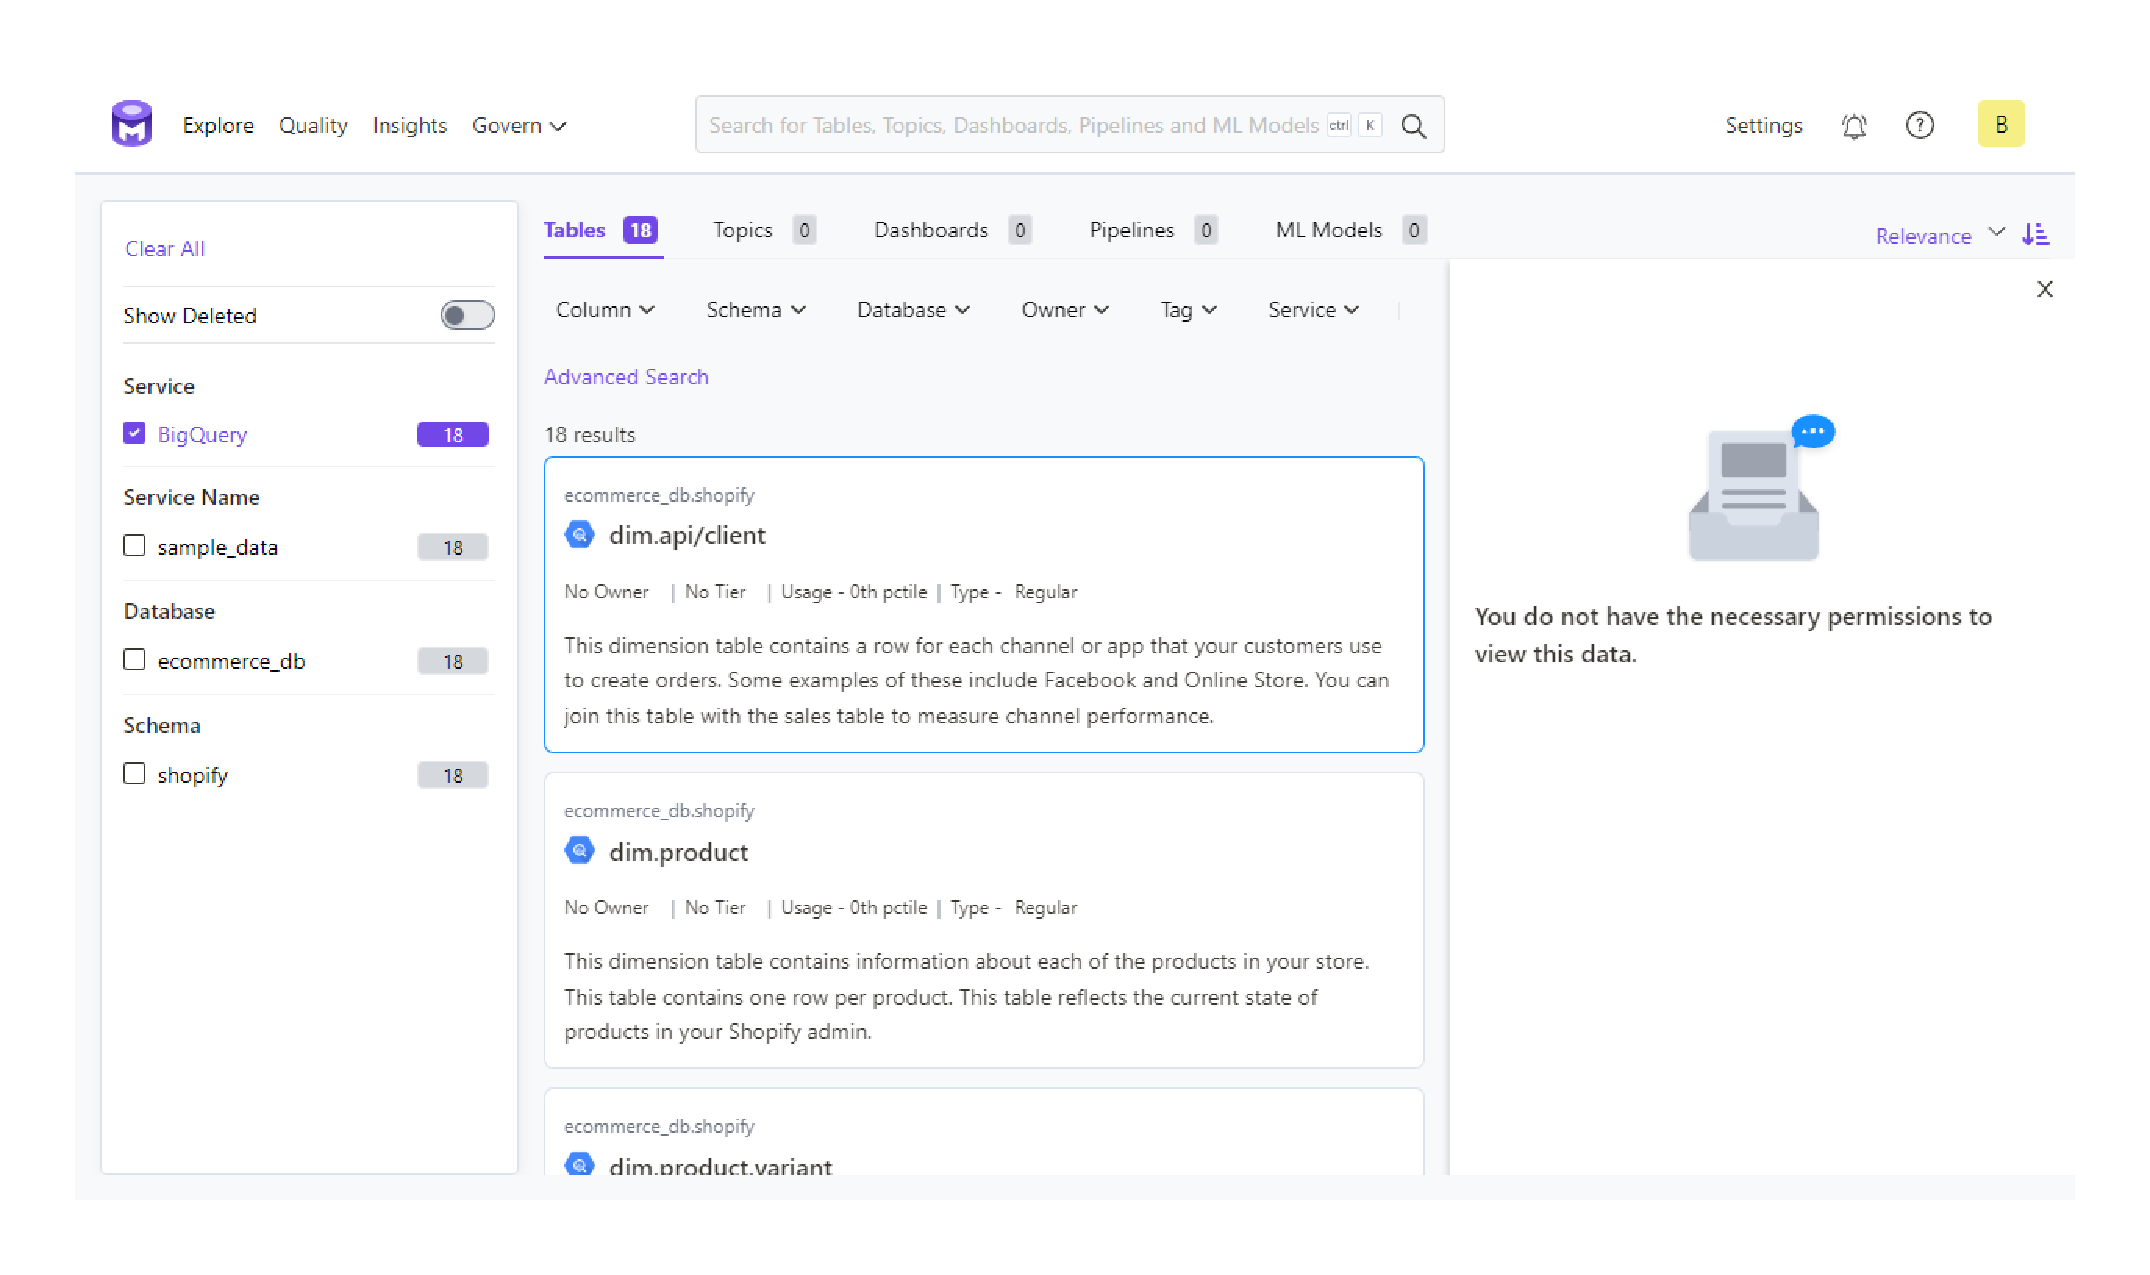
\includegraphics[width=\textwidth]{chapters/implementation/figures/openmetadata_sample_data_explore_denied.pdf}
    \caption{Screenshot of OpenMetadata's Search page, showing the "Access Denied" side panel.}
    \label{fig:openmetadata_sample_data_explore_denied}
\end{figure}

% \subsection{Build artefacts}

% The build artefacts generated by the OpenMetadata project are a tarball and an RPM file. All compiled Java classes and their dependencies are added to the \mintinline{text}{libs} folder so these can be loaded into the classpath of the Java process. The Ranger authoriser handles loading its classes and dependencies using the shim class.

\section{Changes to Apache Ranger}

Additions to the Apache Ranger source code consist of the OpenMetadata service implementation used by the service type definition, as described in Section \ref{sec:plugins_for_apache_ranger}. We define the \mintinline{java}{RangerServiceOpenmetadata} class, extending the \mintinline{java}{RangerBaseService} base class, which handles the verification of configurations of OpenMetadata services defined in Apache Ranger and the generation of initial policies.

\subsection{Validating configurations}

The configurations passed to the \mintinline{java}{RangerServiceOpenmetadata} class are the endpoint of OpenMetadata's Metadata Service, a username and an access token. These are used by the \mintinline[breaklines]{java}{validateConfig()} function to initialise the OpenMetadata Java client, provided by the \mintinline[breaklines, breakafter=.:]{java}{org.open-metadata:openmetadata-java-client} package, and to send a request to the Metadata Service to verify connectivity. While OpenMetadata supports multiple authentication mechanisms (e.g., username and password, Google \acrshort{sso}, Okta \acrshort{sso}, Amazon \acrshort{sso}), the plugin only support the simplest one, \acrshort{jwt} based authentication, using the token passed as part of the configuration. The function returns a \mintinline{java}{Map<String, Object>} object and should throw a \mintinline{java}{HadoopException} to signal errors; thus, the \mintinline{java}{OpenmetadataClient} class is used to wrap the OpenMetadata libraries and extend the \mintinline{java}{BaseClient} base class, implementing the interface required by Apache Ranger.

\subsection{Generating default policies}

Creating default policies is essential to giving the admin a good user experience and programmatically doing much of the repetitive work of setting up initial policies.
It is important to note here that Ranger uses the "Fail-safe defaults" principal \cite{protectionOfInformationInComputerSystemsSaltzer1975} - access is only permitted if it is deliberately granted - meaning a newly set up service instance will block all access. Apache Ranger also follows the principle of "Least privilege" \cite{protectionOfInformationInComputerSystemsSaltzer1975}, but the system does not enforce this; instead, it is the responsibility of the policy administrator. There is an exception to this - the creation of the default policies, where the system is, at the time a new service instance is created, the policy maker. The admin has the full power to delete or completely change default policies, but these should strive to set a good example.

The default mechanism in Apache Ranger for generating policies, implemented by the \mintinline{java}{RangerBaseService.getDefaultRangerPolicies} function, creates a policy for every resource, each with a single rule, allowing all accesses for the group \mintinline{text}{public}. It should be noted that this is configurable, using the \mintinline[breaklines, breakafter=.]{python}{Ranger.default.policy.groups} configuration key for the Ranger Admin Service application and the \mintinline[breaklines, breakafter=.]{python}{default.policy.groups} configuration key for the service instance configuration, but this behaviour is undocumented. Thus, in most practical cases, default policies enable all access for all users.

The OpenMetadata plugin overrides the functionality provided by \mintinline[breaklines, breakbefore=BS]{java}{RangerBaseService} class, following two principles: apply fail-safe defaults, so all access is blocked when the service is created, and give the admins an easy way of privileging users in bulk. Apache Ranger's roles system is employed to facilitate the latter.

To produce the default policies for every resource defined in the service definition, four policies, each assigned to one group:
\begin{itemize}
    \item \textbf{Data-consumer} - allowed any View operation. This is the most common type of user, which can only view resources and not change them;
    \item \textbf{Data-steward} - allowed any View operation and allowed to edit descriptions, names, owners, tags and lineage. These users are the maintainers of the metadata;
    \item \textbf{Bot} - allowed any operation except to create or delete bots or webhooks. Bots are used for automatic operations or service-to-service communication;
    \item \textbf{Admin} - allowed any operation.
\end{itemize}
    \chapter{Experiments and Evaluation}
    \chapter{\label{cha:conclusion}Conclusions}

    %% Print bib 
    \printbibheading
    \printbibliography[nottype=online, heading=subbibliography, title={Academic Resources}]
    \printbibliography[type=online, notkeyword=tech, heading=subbibliography, title={Online Resources}]
    \printbibliography[type=online, keyword=tech, heading=subbibliography, title={Technical Resources}]

    %% Appendices start here
    \appendix
    \chapter{Apache Ranger service definition for OpenMetadata services}
\label{cha:servicedef_full} 

\inputminted[frame=single,
   framesep=3mm,
   linenos=true,
   tabsize=4,
   breaklines,
   breakafter=.,]
{json}
{chapters/appendix/files/ranger-servicedef-openmetadata.json}

\end{document}